\section{Из чего состоит компьютер}\label{base:introduction:components}
\subsection{Общий обзор}\label{base:introduction:components:review}
Рассмотрим типичный персональный компьютер. В общем случае он состоит из устройства вывода изображения (монитор), большой шумящей коробки (системный блок) и разных устройств поменьше.
\begin{figure}[h!]
 \centering
 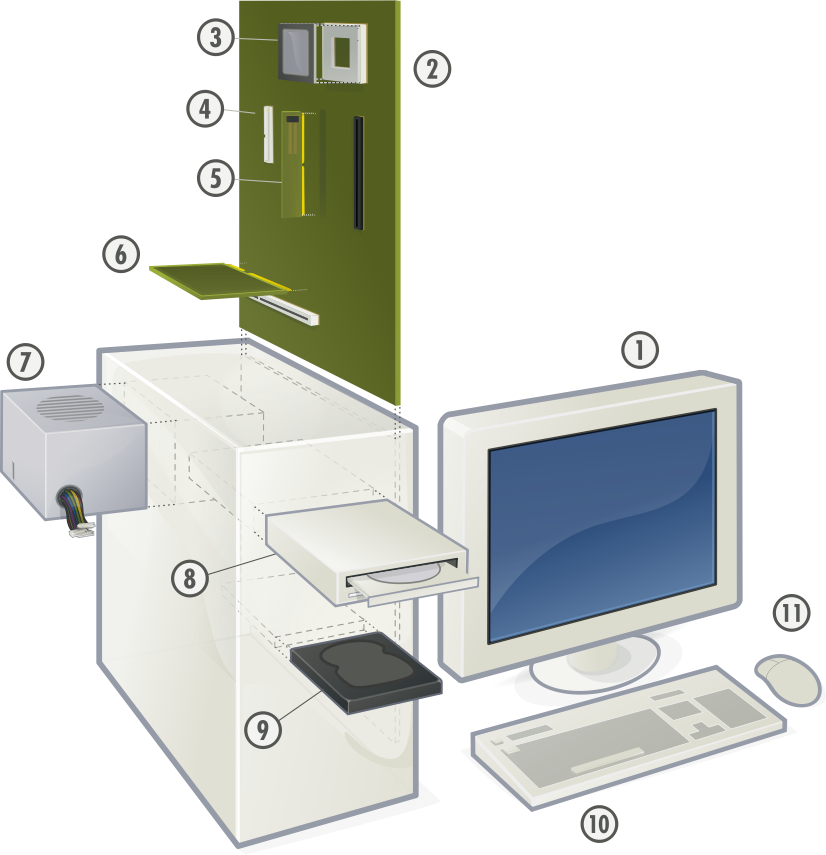
\includegraphics[width=0.5\textwidth]{base/Introduction/Computer.png}
 \label{base:introduction:components:review:computerpic}
 \caption{Устройство персонального компьютера:}
 \footnotesize
 \begin{enumerate}
  \item монитор;
  \item материнская плата;
  \item процессор;
  \item порт ATA;
  \item оперативная память;
  \item карты расширений;
  \item блок питания;
  \item дисковод;
  \item жёсткий диск;
  \item клавиатура;
  \item компьютерная мышь;
 \end{enumerate}
\end{figure}

\subsection{Системный блок}\label{base:introduction:components:case}
Начнём наше знакомство с наиболее заметного компонента настольного компьютера --- \emph{системного блока} (англ.~\emph{computer case} или \emph{computer chassis}). Сам по себе системный блок (по какой-то совершенно неясной причине иногда называемый <<процессором>>; наука пытается найти объяснение этому явлению) является корпусом, в котором располагаются все основные компоненты.
\begin{figure}[h!]
 \centering
 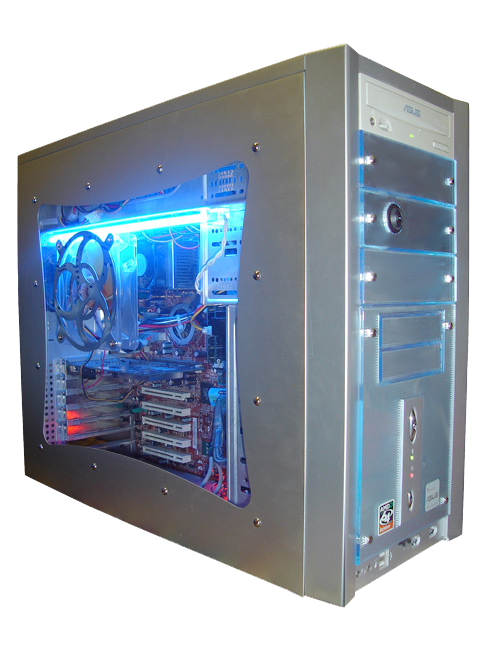
\includegraphics[width=0.5\textwidth]{base/Introduction/Case.png}
 \caption{Типичный системный блок}
 \label{base:introduction:components:case:typicalcasepic}
\end{figure}
\begin{figure}[h!]
 \centering
 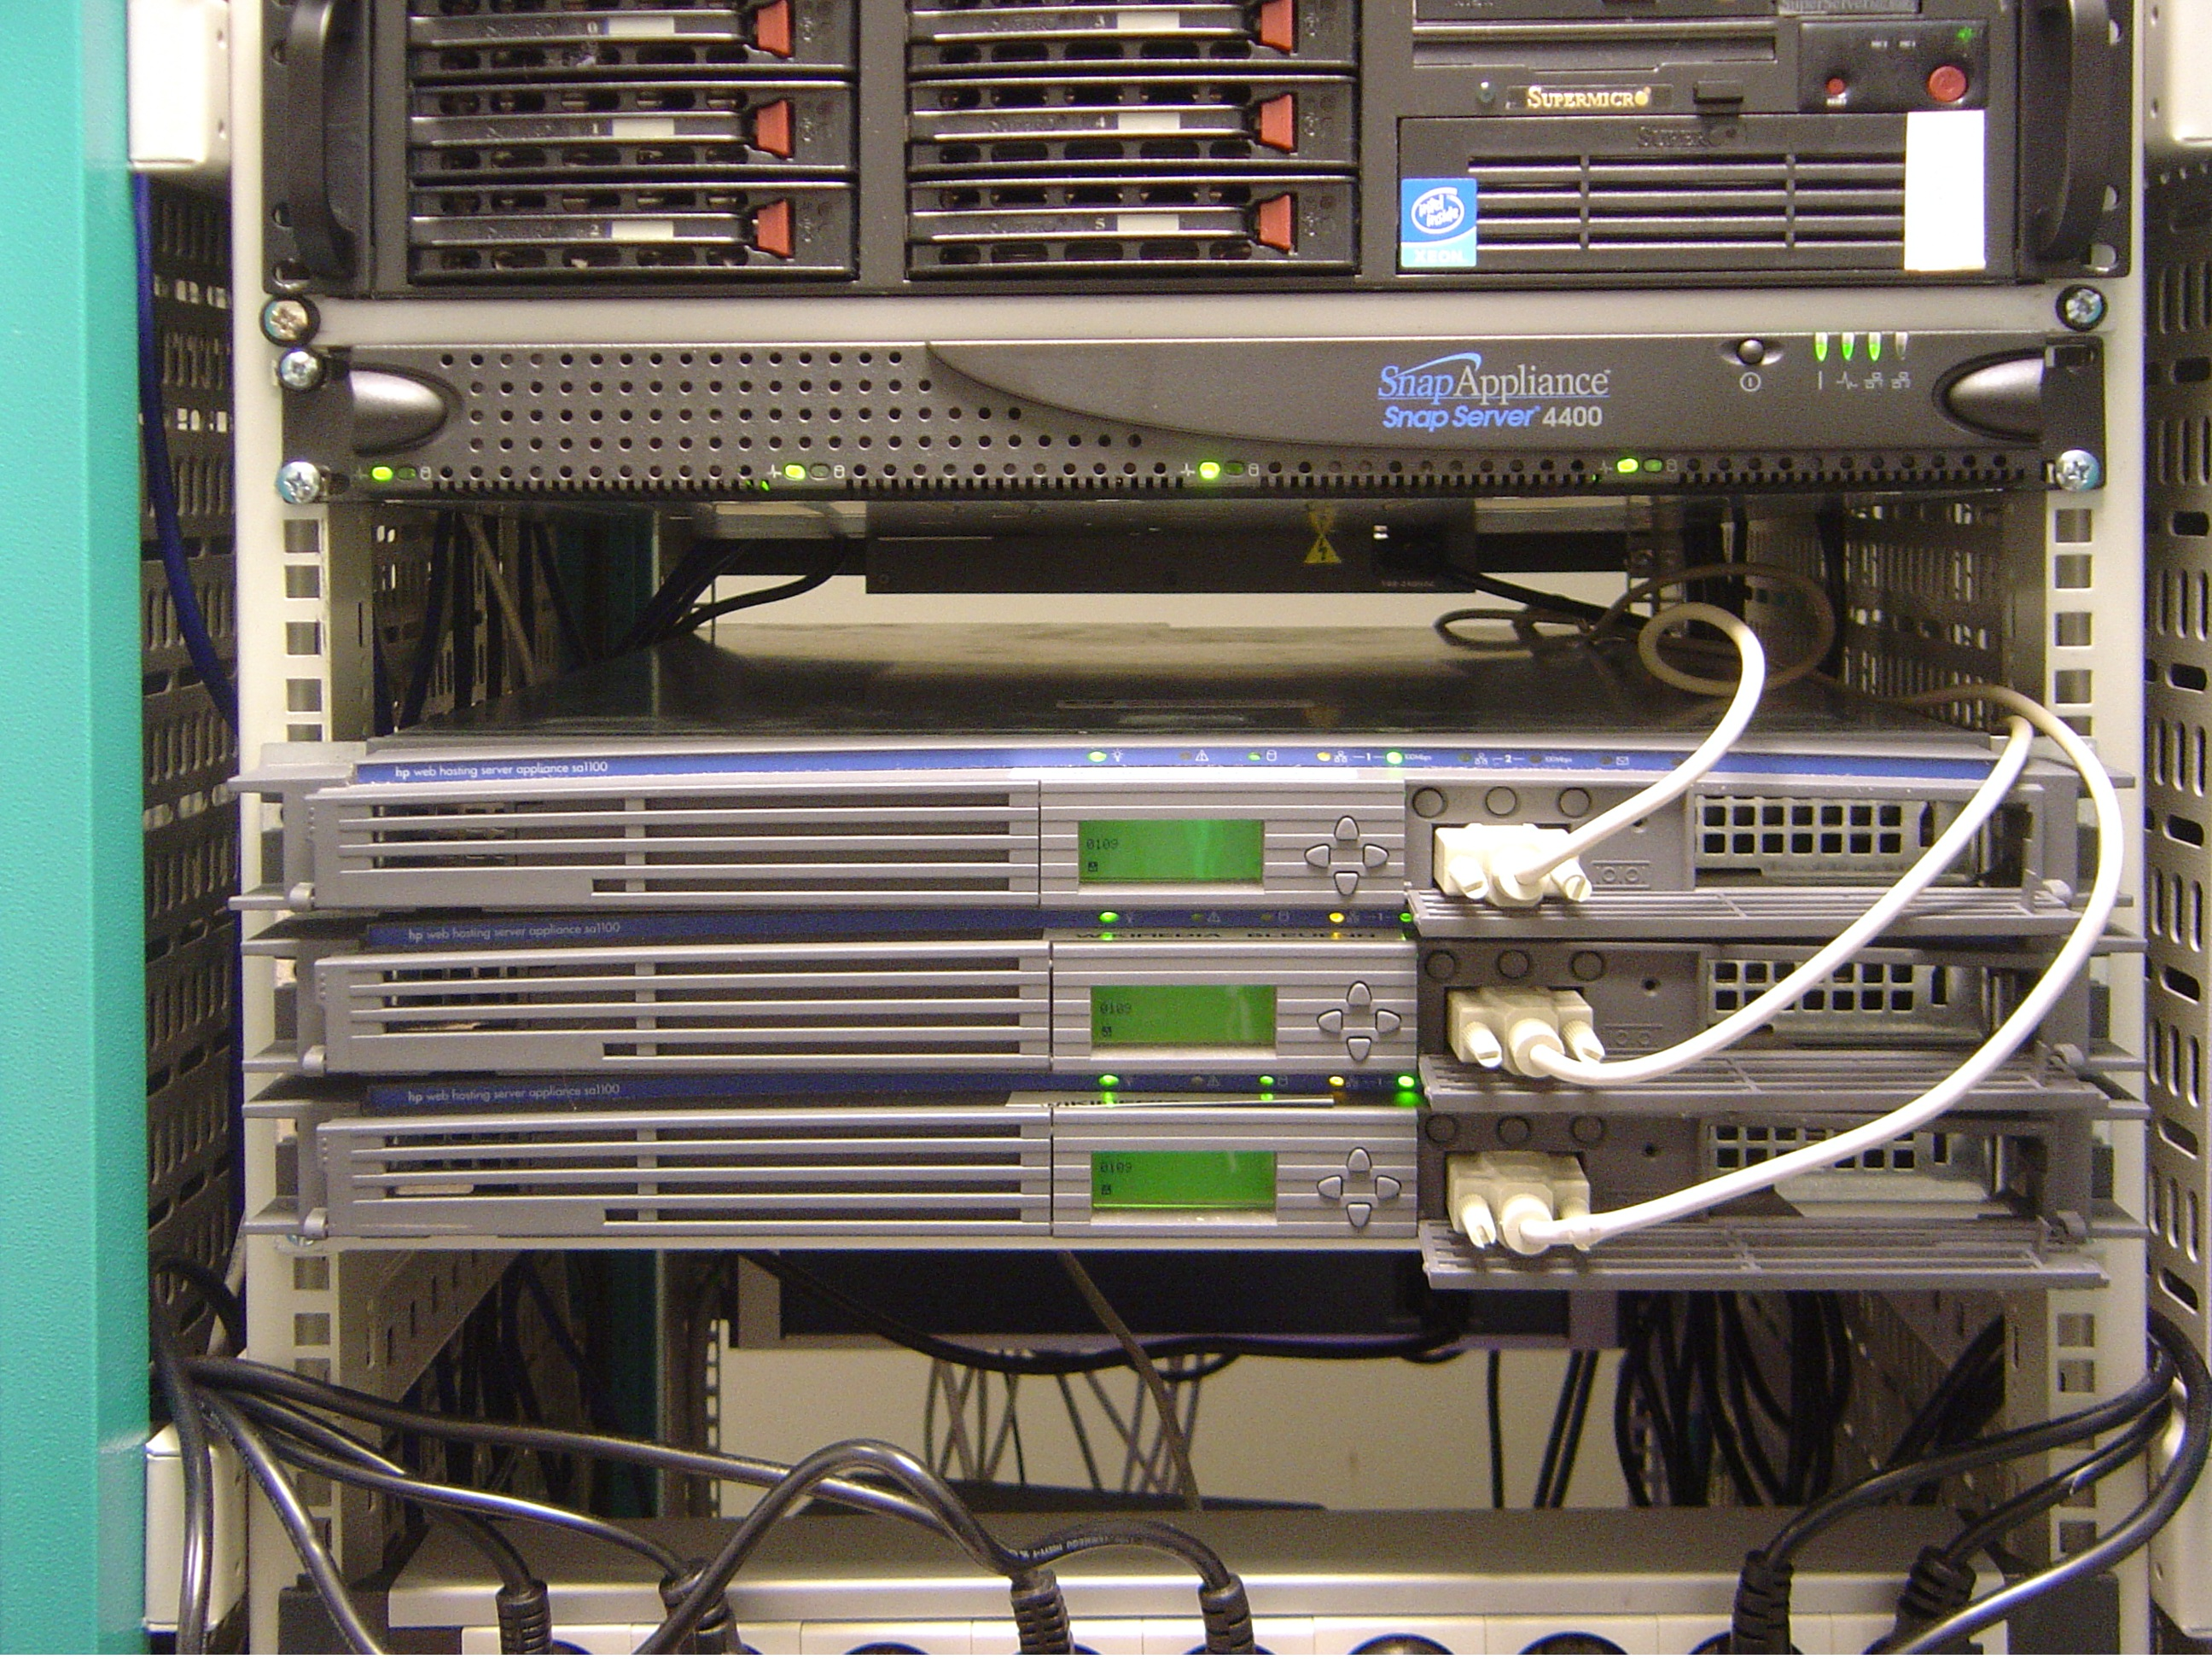
\includegraphics[width=0.5\textwidth]{base/Introduction/Case_wikipedia.jpg}
 \caption{Корпуса серверов Википедии}
 \label{base:introduction:components:case:wikipediacasepic}
\end{figure}
Внутреннее пространство поделено на несколько секций: отсек под устройства формата 5,25 дюймов, отсек под устройства формата 3,5 дюйма, место крепления блока питания и место для крепления материнской платы.

Корпуса могут быть разных форм и размеров. Относительно пропорций есть два устоявшихся форм-фактора: горизонтальные и вертикальные. Среди горизонтальных форм-факторов можно отметить:
\begin{description}
 \item[Desktop] $533\times419\times152$\,мм
 \item[FootPrint] $406\times406\times152$\,мм
 \item[SlimLine] $406\times406\times101$\,мм
 \item[UltraSlimLine] $381\times352\times75$\,мм
\end{description}
Также к горизонтальным форм-факторам можно причислить стоечные корпуса.

Вертикальные форм-факторы встречаются наиболее часто в офисах, домах, компьютерных классах. Они объединены общим названием \emph{Tower} (minitower, miditower, bigtower). Среди причин их распространённости можно отметить больший объём по сравнению с горизонтальными, за счёт чего внутри остаётся больше места для вентиляции или дополнительных компонентов.

Вне зависимости от форм-фактора, системный блок является своеобразной <<печкой>>. Для охлаждения устройств, расположенных в нём, используется система вентиляции или циркуляции охлаждённой жидкости. Вентиляцию обеспечивают специальные вентиляторы (\emph{кулеры}, англ. \emph{cooler}), расположенные как на наиболее тепловыделяющих уст\-ройствах, так и на самом корпусе.
Довольно часто кулеры ставятся парно и однонаправлено, таким образом получается, что один задумает воздух внутрь, а другой выдувает наружу. За счёт этого обеспечивается постоянный поток воздуха, который оказывает охлаждающее действие.
Также кулеры устанавливают на одну из боковых стенок вертикальных форм-факторов, и иногда на вертикальные. Т.\,к.~охлаждение --- необходимый для нормального функционирования компьютера процесс, к его осуществлению надо подходить очень внимательно.
В частности, представляется недопустимым помещение системных блоков в тестные ниши современных компьютерных столов, т.\,к.~ограниченность пространства этих ниш делает задачу охлаждения труднорешаемой, а установленные средства воздушного охлаждения --- малоэффективными.

\subsubsection{Центральный процессор}\label{base:introduction:components:cpu}
Теперь рассмотрим \emph{центральный процессор} --- главное управляющее устройство, исполняющее машинные инструкции.
Изначально термин <<центральное процессорное устройство>> описывал специализированный класс логических машин, предназначенных для выполнения сложных компьютерных программ.
Вследствие довольно точного соответствия этого назначения функциям существовавших в то время компьютерных процессоров, он естественным образом был перенесён на сами компьютеры.
Начало применения термина и его аббревиатуры по отношению к компьютерным системам было положено в 1960-е годы.
Устройство, архитектура и реализация процессоров с тех пор неоднократно менялись, однако их основные исполняемые функции остались теми же, что и прежде.

\begin{figure}[h!]
 \centering
 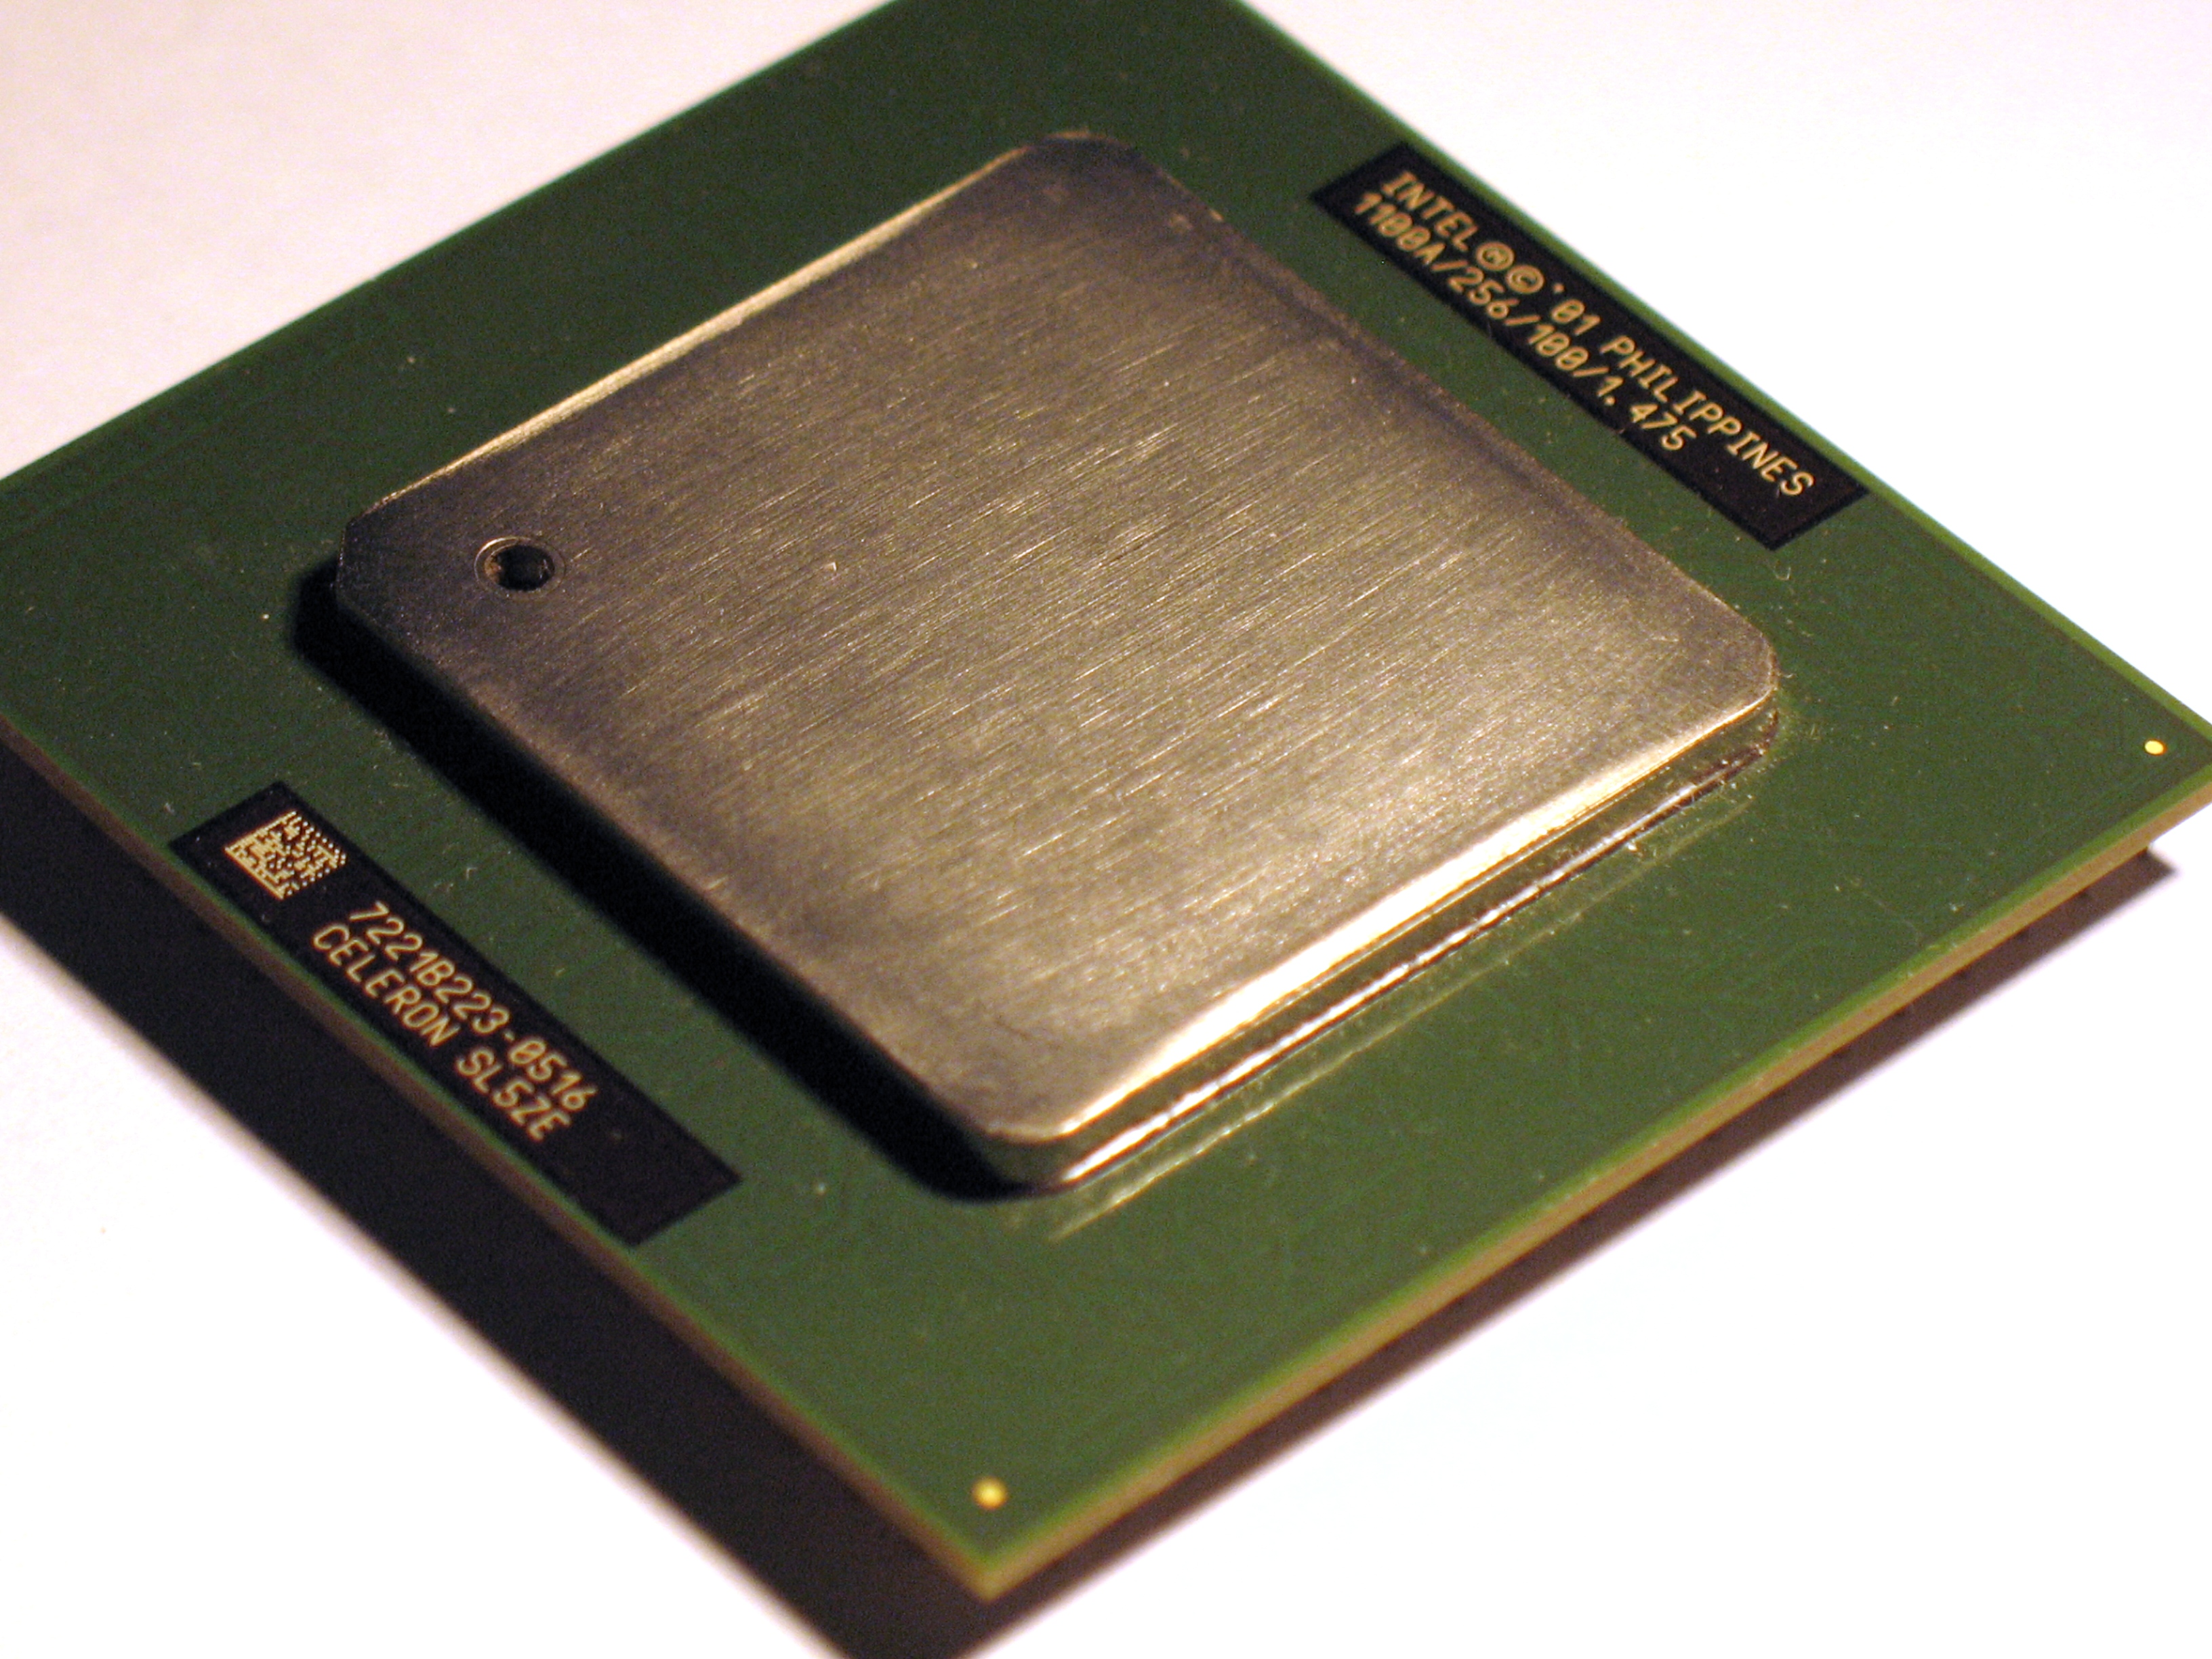
\includegraphics[width=0.33\textwidth]{base/Introduction/CPUup.jpg}
 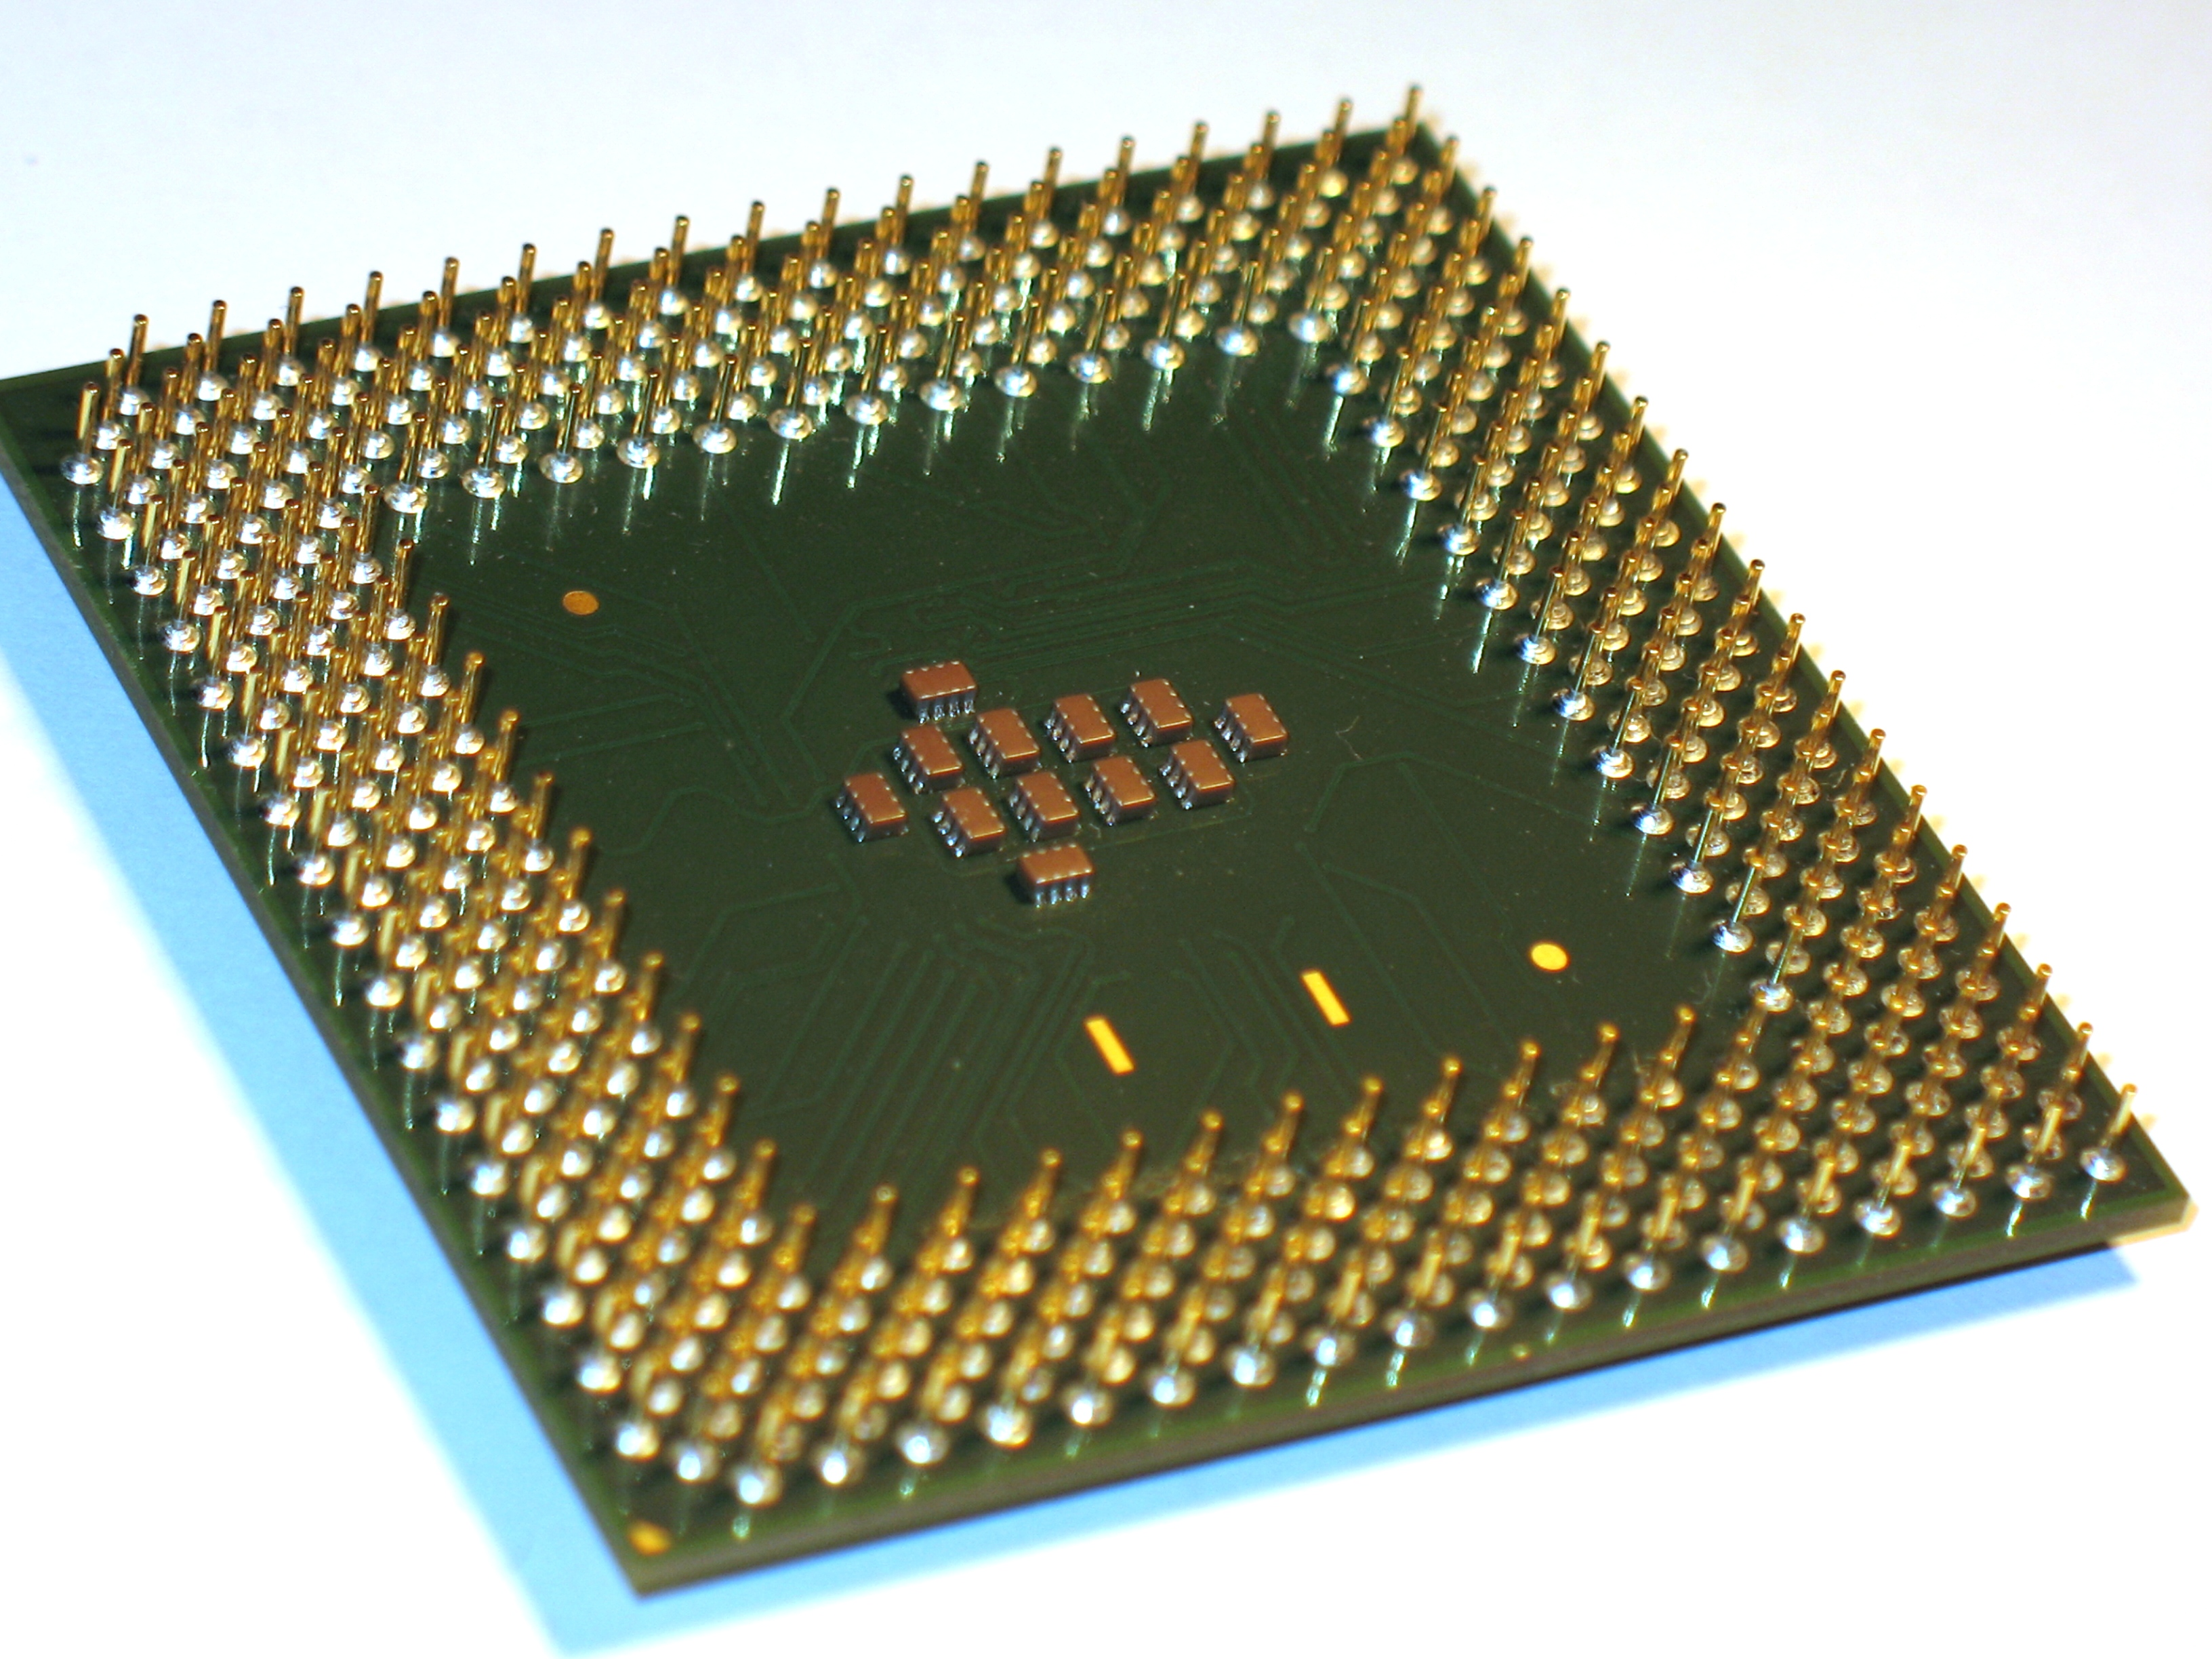
\includegraphics[width=0.33\textwidth]{base/Introduction/CPUdown.jpg}
 \label{base:introduction:components:cpu:cpupic}
 \caption{Центральный процессор}
\end{figure}

Главными характеристиками ЦПУ являются: \emph{тактовая частота}, \emph{производительность}, \emph{энергопотребление}, \emph{архитектура} и \emph{нормы литографического производственного процесса}. Рассмотрим их поподробнее:

\textbf{Производительность} --- это количественная характеристика скорости выполнения определённых операций на компьютере.
Чаще всего вычислительная мощность измеряется во флопсах (количество операций с плавающей запятой в секунду), а также производными от неё.
На данный момент принято причислять к суперкомпьютерам системы с вычислительной мощностью более 10 Терафлопс ($10\times10^{12}$ или десять триллионов флопс; для сравнения среднестатистический современный настольный компьютер имеет производительность порядка 0,1 Терафлопс).

Существует несколько сложностей при определении вычислительной мощности компьютера.
Во-первых, следует иметь в виду, что производительность системы может сильно зависеть от типа выполняемой задачи.
В частности, отрицательно сказывается на вычислительной мощности необходимость частого обмена данных между составляющими компьютерной системы, а также частое обращение к памяти.
В связи с этим выделяют \emph{пиковую вычислительную мощность} --- гипотетически максимально возможное количество операций над числами с плавающей запятой в секунду, которое способен произвести данный компьютер.

\textbf{Тактовая частота} --- как следует из названия, определяет количество тактов, выполняемых за секунду. Условно можно переопределить это понятие как <<количество инструкций в секунду>>.
Среди потребителей имеется распространённое заблуждение о том, что процессоры с более высокой тактовой частотой всегда имеют более высокую производительность, чем процессоры с более низкой тактовой частотой.
На самом деле это не совсем так, т.\,к.~за один такт на разных процессорах может выполняться разное количество инструкций.

\textbf{Норма литографического процесса} --- описание технического процесса при производстве процессора. Наиболее важной характеристикой является разрешающая способность оборудования --- то есть, как следствие, плотность нанесения элементов.

\textbf{Архитектура} процессора --- количественная составляющая компонентов микроархитектуры процессора компьютера (например, регистр флагов или регистры процессора), рассматриваемая IT-специалистами в аспекте прикладной деятельности.
С точки зрения программиста --- совместимость с определённым набором команд, их структуры и способа исполнения.
С точки зрения аппаратной составляющей вычислительной системы --- это некий набор свойств и качеств, присущий целому семейству процессоров.
Имеются различные классификации архитектур процессоров, как по организации (например, по количеству и скорости выполнения команд: RISC, CISC), так и по назначению (например, специализированные графические).

\subsubsection{Оперативная память}\label{base:introduction:components:ram}
\begin{figure}[h!]
 \centering
 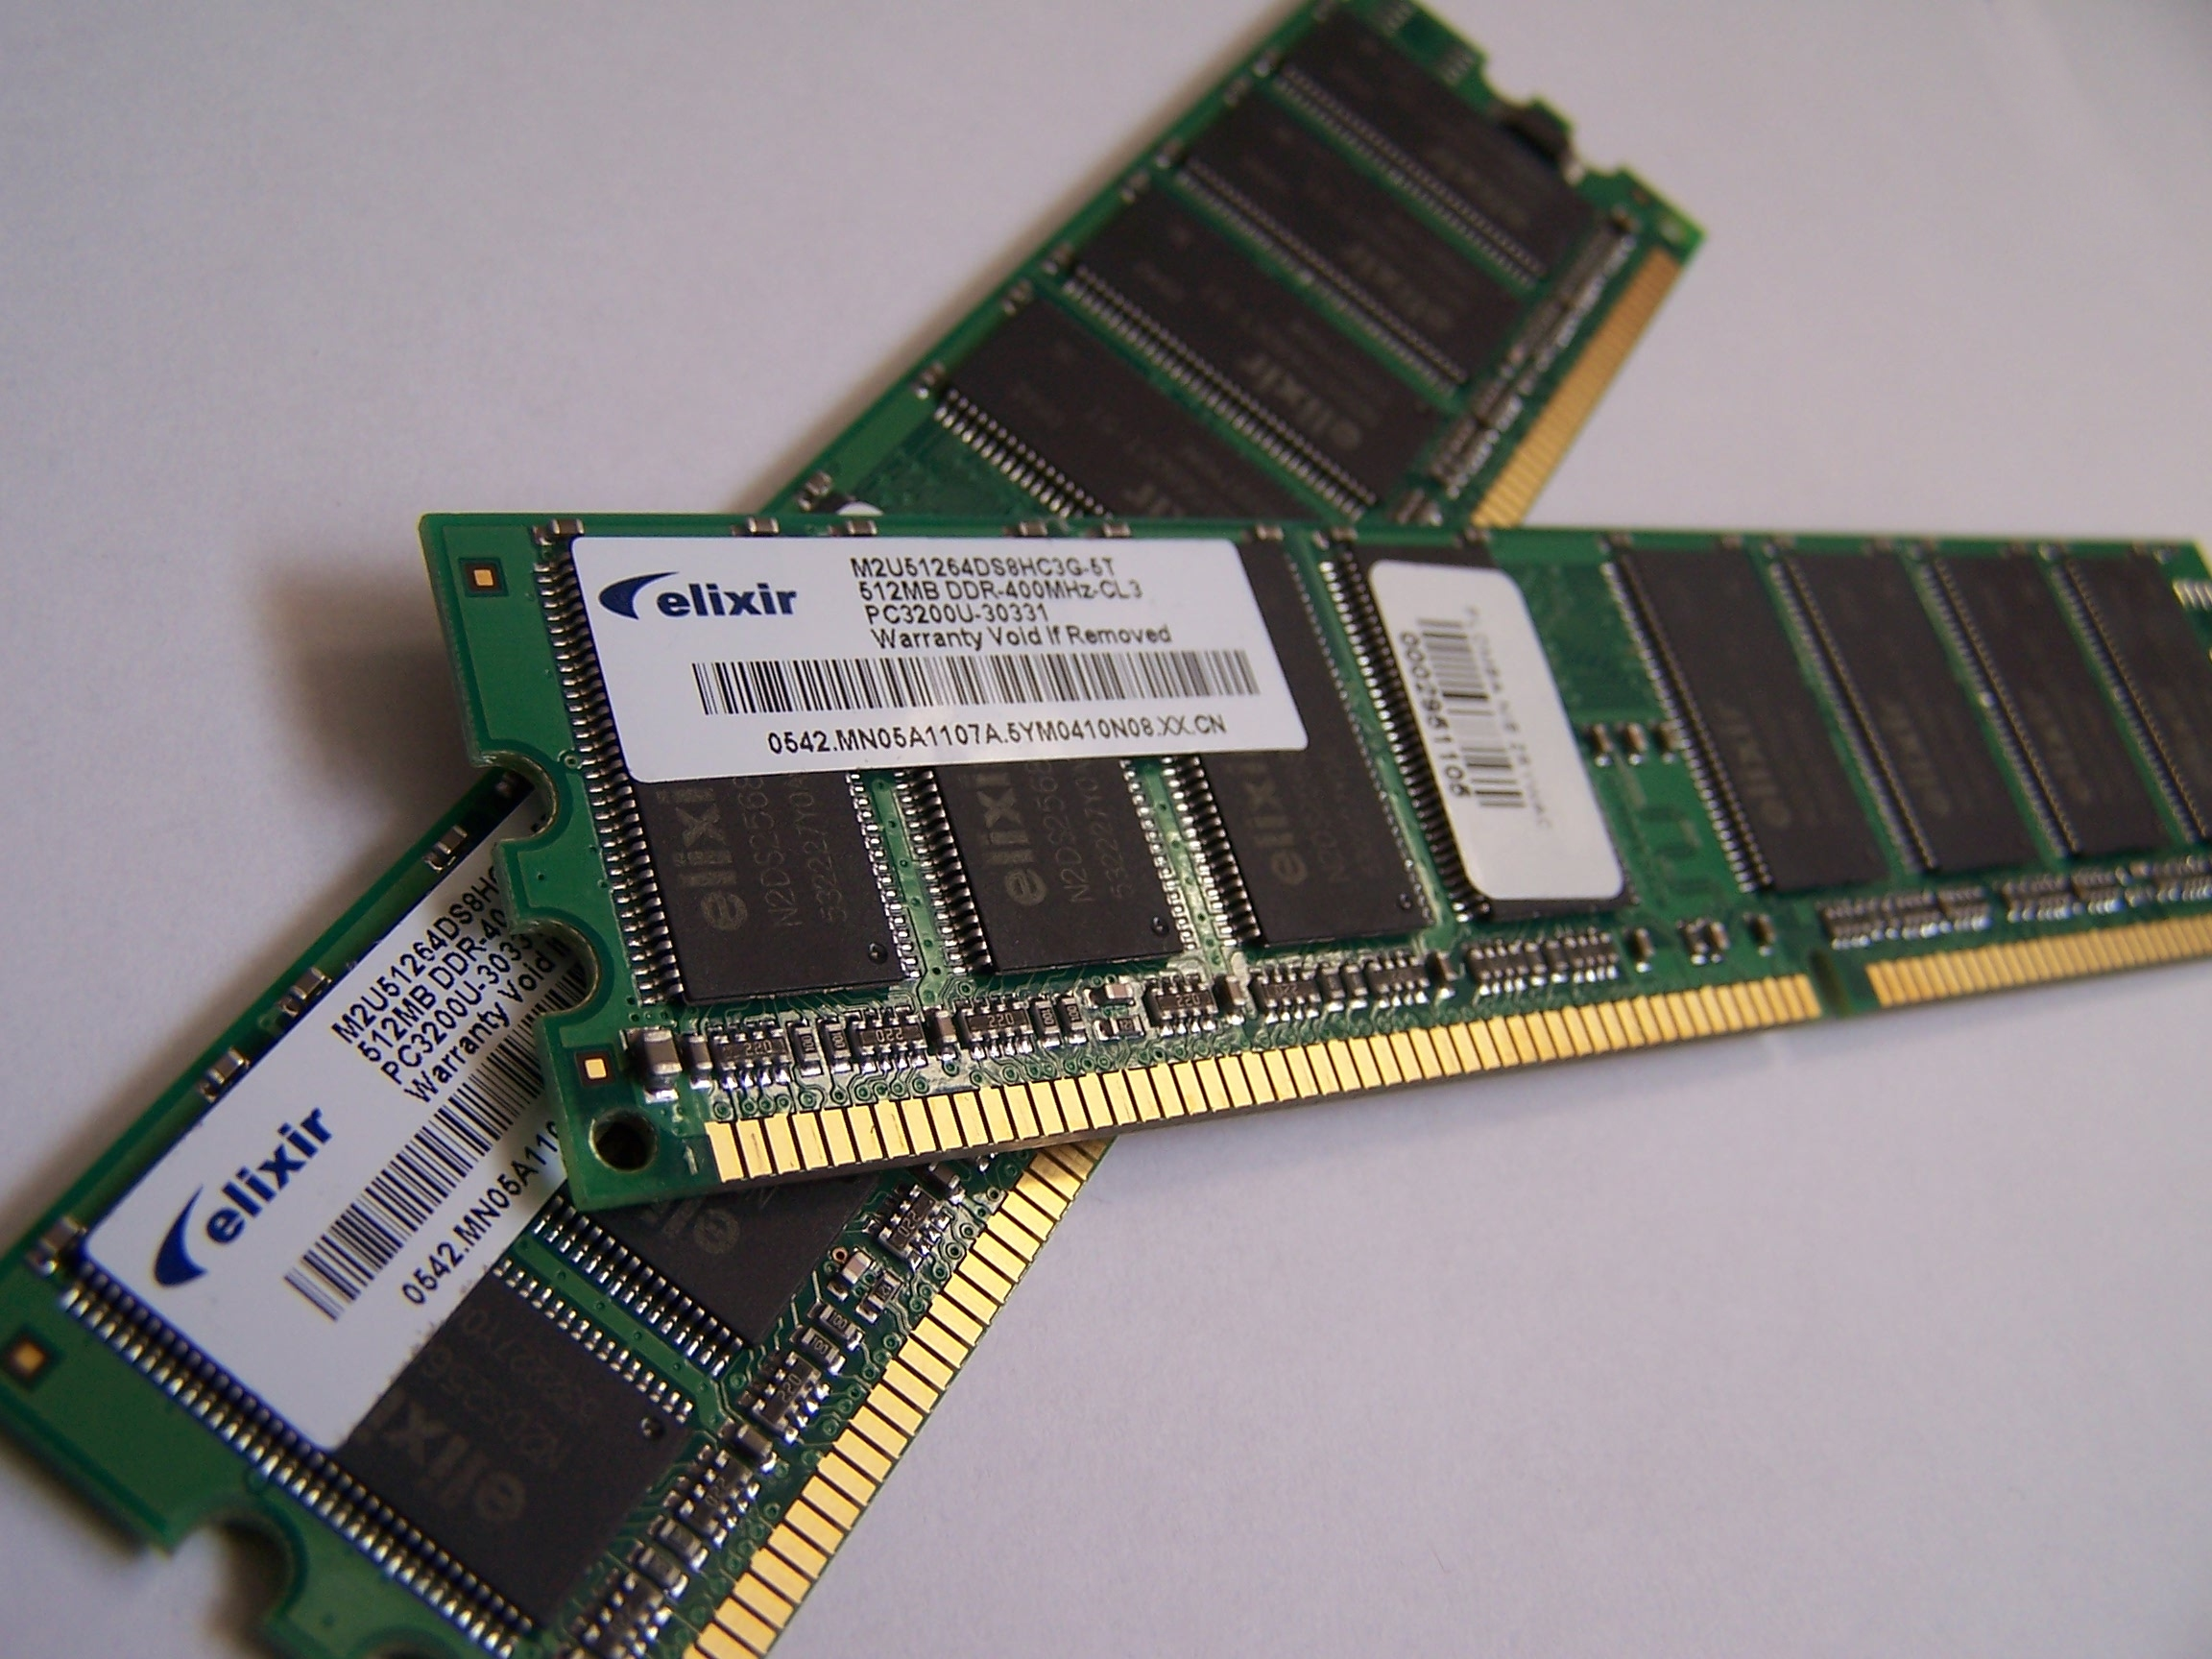
\includegraphics[width=0.5\textwidth]{base/Introduction/Memory.jpg}
 \label{base:introduction:components:ram:rampic}
 \caption{Плашки памяти DDRAM}
\end{figure}
\emph{Оперативно запоминающее устройство} --- энергозависимая плата, обеспечивающая временное хранение данных. Также часто синонимом ОЗУ выступает словосочетание <<\emph{оперативная память}>> --- по сути, его основная функция.
В оперативной памяти хранятся данные приложений, операционная система и многое другое.
Именно отсюда центральный процессор берёт инструкции для выполнения, записанные в программе, и именно сюда записывает их результат.
Даже если надо вывести простую строчку текста на экран, эта строчка будет размещена в оперативной памяти, и лишь затем будет считана оттуда для вывода.
Как следствие, к ней идёт постоянное обращение и происходит постоянный обмен данными.
За счёт этого растут требования к скорости памяти, отчего она получила своё название, а вместе с этим и стоимость.
Оперативная память стоит очень дорого (250--1875~руб. за гигабайт у ОЗУ при 1,5--3,75~руб. за гигабайт у жёстких дисков), притом что её использует каждое приложение для хранения данных.

Основными параметрами оперативной памяти являются \emph{объём} и \emph{частота шины}.
В качестве объёма указывается количество данных, которое может быть помещено в память.
Частота шины же показывает, сколько операций может быть совершено за еденицу времени, таким образом плата с большей частотой окажется быстрее платы аналогичного объёма, но с реже обновляемой шиной.
Стоит отметить, что на памяти указывается \emph{максимальная} частота, а не фактическая.
Реальная скорость также зависит от частоты шины на материнской плате, и из двух будет использоваться самая медленная.

У других устройств могут быть свои аналоги оперативной памяти, призванные снизить нагрузку на оную и/или ускорить получение данных.
Например, в процессорах, особенно в центральном, имеется \emph{кеш-память}, обладающая огромной скоростью даже по сравнению с оперативной, куда записываются самые частоиспользуемые инструкции или другие данные, вероятность обращения к которым крайне высока.
Аналогичные по функциям кеши имеют и некоторые другие устройства.
Объём их, как правило, очень мал, что не позволяет использовать их для ускорения работы системы

\subsubsection{Материнская плата}\label{base:introduction:components:motherboard}
\begin{figure}[h!]
 \centering
 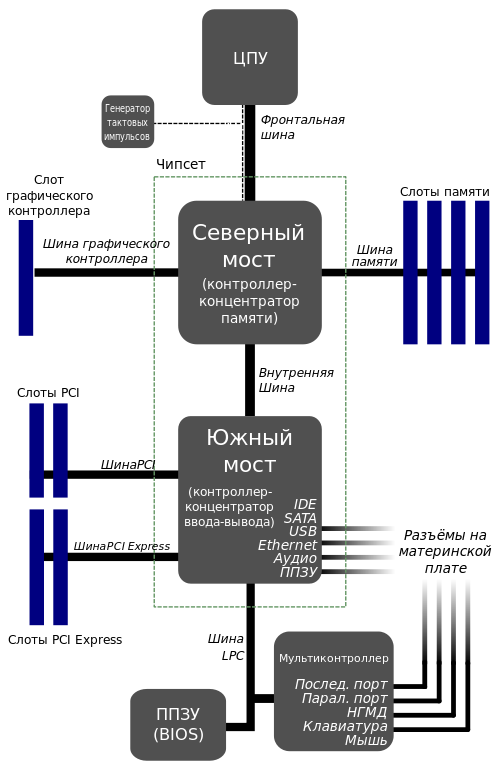
\includegraphics[width=0.9\textwidth]{base/Introduction/Motherboard_diagram.png}
 \caption{Схема устройства материнской платы}
 \label{base:introduction:components:motherboard:diagrampic}
\end{figure}
\begin{figure}
 \centering
 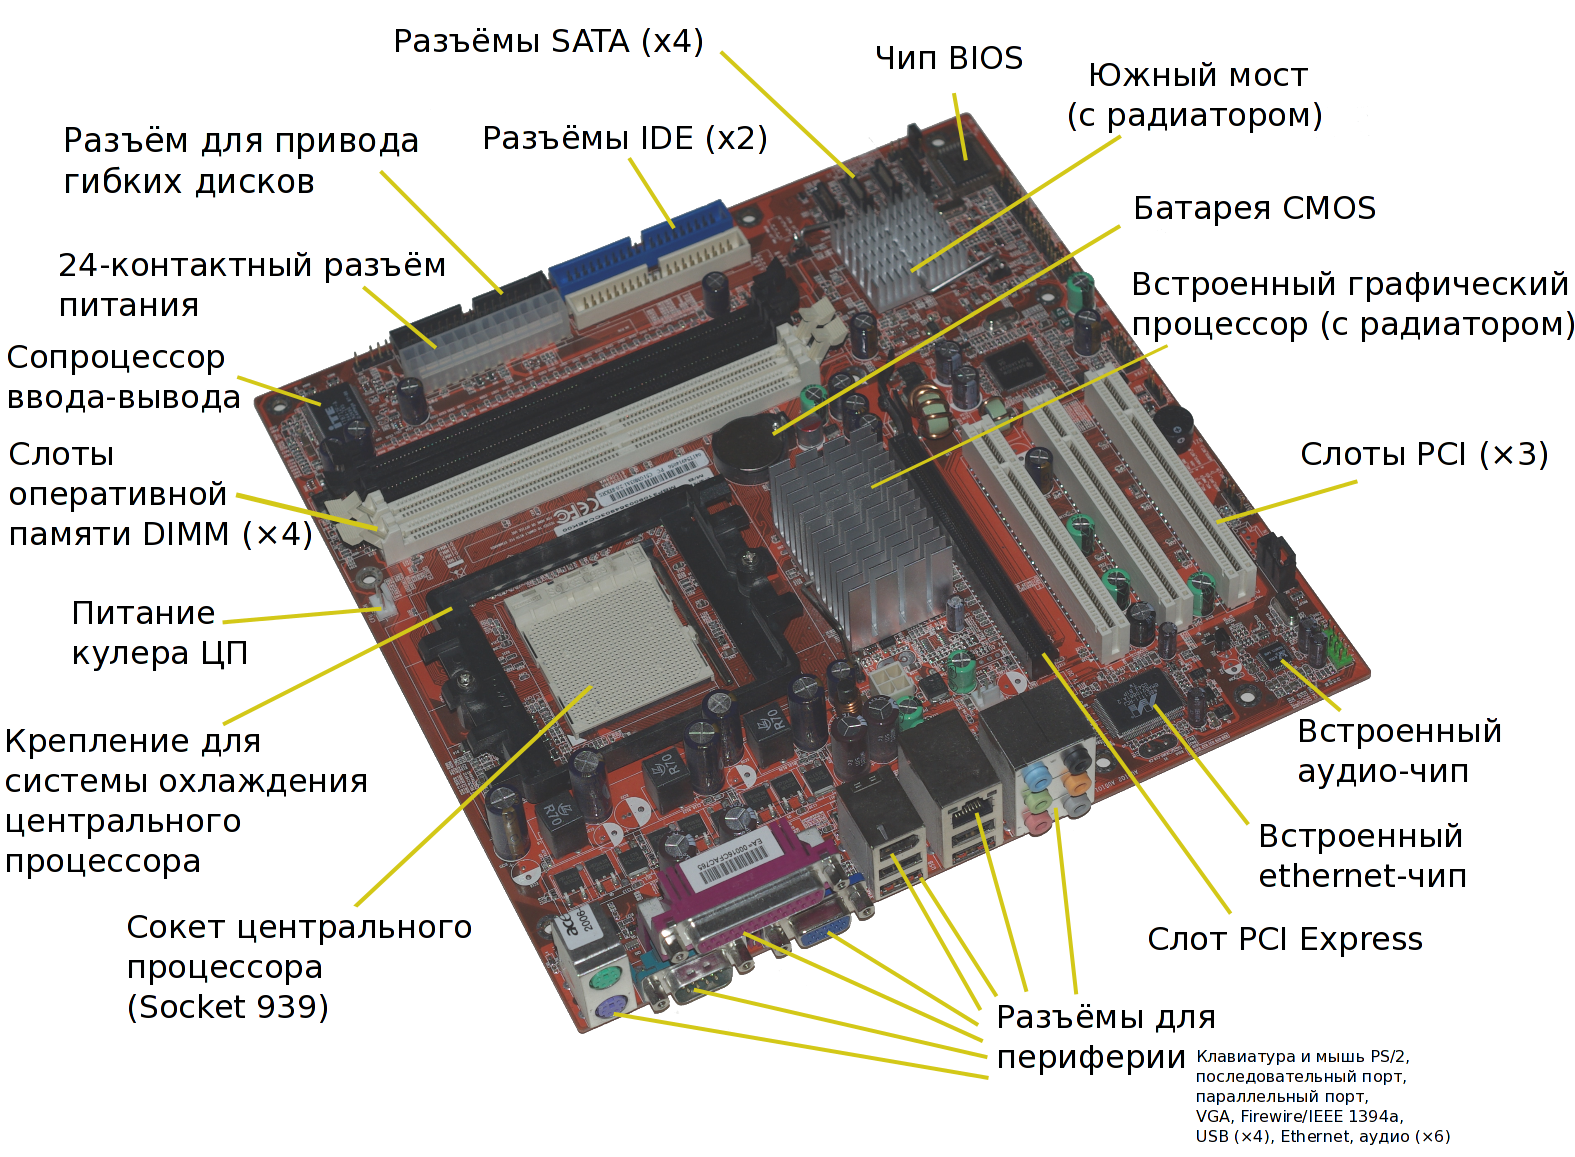
\includegraphics[width=\textwidth]{base/Introduction/Motherboard.png}
 \label{base:introduction:components:motherboard:motherboardpic}
\end{figure}
Следующей рассмотрим основную плату компьютера, соединяющую всё воедино.
\emph{Материнская плата} (англ. \emph{motherboard}, \emph{MB}) --- сложная многослойная печатная плата, на которой устанавливаются основные компоненты персонального компьютера.
Именно материнская плата объединяет и координирует работу таких различных по своей сути и функциональности комплектующих, как процессор, оперативная память, платы расширения и всевозможные накопители.

Современные материнские платы содержат, как минимум:
\begin{itemize}
 \item сокет для ЦПУ;
 \item слоты для оперативной памяти;
 \item \emph{чипсет} (англ. \emph{chipset}), являющийся основным средством взаимодействия между устойствами;
 \item энергонезависимую память, хранящую BIOS и прочее необходимое ПО;
 \item тактовый генератор, используемый для синхронизации различных компонентов;
 \item слоты расширения;
 \item разъёмы для подключения внешнего источника питания, а также разъёмы для обеспечения питанием некоторых устройств (например, кулер ЦПУ).
\end{itemize}

Также, почти все материнские платы включают логику и разъёмы для поддержки часто используемых устройств ввода, таких как PS/2 для подключения мыши и клавиатуры.
Иногда они могут содержать графические интерфейсы и простые графические процессоры.
Дополнительная периферия, такая как дисковые контроллеры, может быть представлена платами расширения.

Учитывая большое тепловыделение быстрых процессоров и прочих устройств, современные материнские платы имеют радиаторы и точки для крепления дополнительных вентиляторов.

Чипсет --- это набор системной логики, набор микросхем, обеспечивающих подключение ЦПУ к ОЗУ и контроллерам периферийных устройств.
Как правило, современные наборы системной логики строятся на базе двух схем: <<северного>> и <<южного мостов>>.

\emph{Северный мост} (англ. \emph{Northbridge}), \emph{MCH} (\emph{Memory controller hub}), \emph{системный контроллер} --- обеспечивает подключение ЦПУ к узлам, использующим высокопроизводительные шины: ОЗУ, графический контроллер.
Обычно к системному контроллеру подключается ОЗУ, в этом случае он содержит в себе контроллер памяти.
Таким образом, от типа применённого системного контроллера обычно зависит максимальный объём ОЗУ, а также пропускная способность шины памяти персонального компьютера.
Однако в настоящее время имеется тенденция встраивания контроллера ОЗУ непосредственно в центральный процессор, что упрощает функции системного контроллера и снижает тепловыделение.
В качестве шины для подключения графического контроллера на современных материнских платах используется PCI Express.
Ранее использовались общие шины (ISA, VLB, PCI) и шина AGP.

\emph{Южный мост} (англ. \emph{Southbridge}), \emph{ICH} (\emph{I/O controller hub}), \emph{периферийный контроллер} --- содержит контроллеры периферийных устройств (таких как жёсткого диска, Ethernet, аудио), контроллеры шин для подключения периферийных устройств (шины PCI, PCI Express и USB), а также контроллеры шин, к которым подключаются устройства, не требующие высокой пропускной способности.

\subsubsection{Видеокарта}\label{base:introduction:components:videocard}
\begin{figure}[h!]
 \centering
 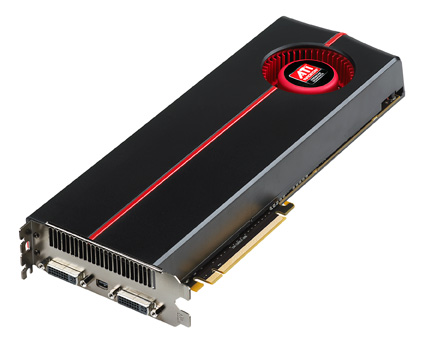
\includegraphics[width=0.5\textwidth]{base/Introduction/Videocard.jpg}
 \caption{Видеокарта}
 \label{base:introduction:components:videocard:videocardpic}
\end{figure}
Перейдём к платам расширения и начнём с одной и самых важных --- \emph{видеокарты}.
Видеокарта (\emph{графический адаптер}) преобразует графический образ, хранящийся в памяти компьютера или самого адаптера, в форму, пригодную для дальнейшего вывода на экран монитора.
В настоящее время, однако, эта базовая функция утратила основное значение, и, в первую очередь, под графическим адаптером понимают устройство с \emph{графическим процессором} --- \emph{графический ускоритель}, который и занимается формированием самого графического образа.
Современные видеокарты не ограничиваются простым выводом изображения, они имеют встроенный графический процессор, который может производить дополнительную обработку, снимая эту задачу с центрального процессора компьютера.
В последнее время также имеет место тенденция использовать вычислительные возможности графического процессора для решения неграфических задач.

Видеоускоритель может быть также интегрирован в материнскую плату или (с недавних пор) центральный процессор, однако все материнские платы настольных компьютеров имеют слот расширения под отдельную плату.
Современные компьютеры низшего и среднего классов часто содержат графический чипсет, расположенный на северном мосту материнской платы.
Эти графические чипы обычно содержат небольшой объём памяти (или не содержат её вовсе) и резервируют для своих нужд часть оперативной памяти, уменьшая её доступный остальным компонентам объём и приводя к ограничениям производительности, так как и центральный и графический процессоры для доступа к памяти используют одну шину.

Интегрированные видеокарты подразделяются на следующие категории:
\begin{itemize}
 \item \emph{Графика с разделяемой памятью} (\emph{Shared graphics}, \emph{Shared Memory Architecture}).
  Видеопамять в виде специализированных ячеек как таковая отсутствует; вместо этого под нужды видеоадаптера динамически выделяется область основной оперативной памяти компьютера.
  Такой способ адресации памяти почти исключительно используют т.\,н.~интегрированные видеокарты (т.\,е.~выполненные не в виде отдельной микросхемы, а являющиеся частью одного большого чипа --- северного моста).
  Преимущества данного решения --- низкая цена и малое энергопотребление.
  Недостатки --- невысокая производительность в 3D-графике и меньшая пропускная способность памяти.
 \item \emph{Дискретная графика} (\emph{Dedicated graphics}).
  На системной плате или (реже) на отдельном модуле распаяны видеочип и один или больше модулей видеопамяти.
  Только дискретная графика обеспечивает наивысшую производительность в трёхмерной графике.
  Недостатки: более высокая цена (для высокопроизводительных процессоров --- очень высокая) и большее энергопотребление.
 \item \emph{Гибридная дискретная графика} (\emph{Hybrid graphics}).
  Как следует из названия --- комбинация вышеназванных способов, ставшая возможной с появлением шины PCI Express.
  Наличествует небольшой объём физически распаянной на плате видеопамяти, который может виртуально расширяться за счёт использования основной оперативной памяти.
  Компромиссное решение, с разной степенью успеха пытаеющееся нивелировать недостатки двух вышеназванных видов, но не устраняет их полностью.
\end{itemize}

Среди характеристик видеоадаптеров следует выделить следующие:
\begin{itemize}
 \item \emph{ширина шины памяти}, измеряется в битах --- количество информации, передаваемой за такт.
  Важный параметр в производительности карты;
 \item \emph{объём видеопамяти} --- объём собственной оперативной памяти видеокарты.
  Видеокарты, интегрированные в набор системной логики материнской платы или являющиеся частью ЦПУ, обычно не имеют собственной видеопамяти и используют для своих нужд часть оперативной памяти компьютера;
 \item \emph{частоты ядра} и \emph{памяти} --- чем больше, тем быстрее видеокарта будет обрабатывать информацию;
 \item \emph{текстурная} и \emph{пиксельная скорость заполнения} --- показывает количество выводимой информации в единицу времени.
\end{itemize}

\subsubsection{Звуковая карта}\label{base:introduction:components:soundcard}
\begin{figure}
 \centering
 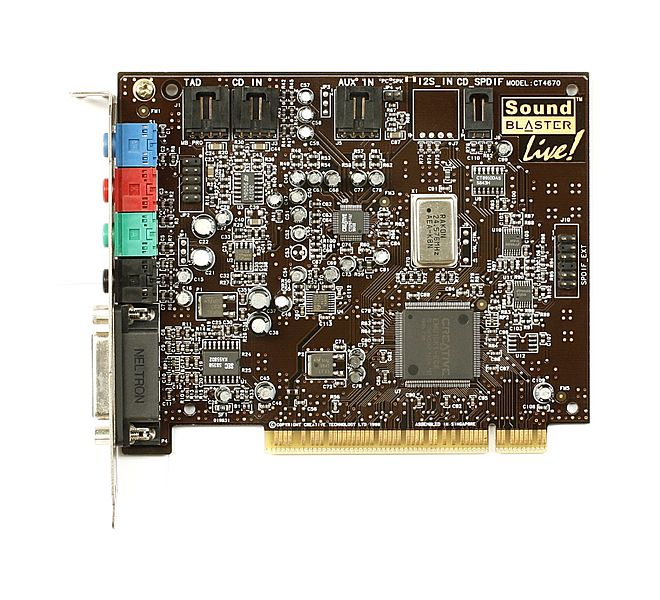
\includegraphics[width=0.5\textwidth]{base/Introduction/Soundcard.jpg}
 \label{base:introduction:components:soundcard:soundcardpic}
 \caption{Звуковая карта}
\end{figure}
\emph{Звуковая карта} (англ. \emph{sound card}) --- дополнительное оборудование персонального компьютера, позволяющее воспроизводить и записывать звук.
На момент появления звуковые платы представляли собой отдельные карты расширения, устанавливаемые в соответствующий слот.
В современных материнских платах представлены в виде интегрированного в материнскую плату аппаратного кодека.

Современные встроенные звуковые карты обеспечивают качество, достаточное для большинства пользователей.  Даже самые низкобюджетные платы могут воспроизводить аудио CD-качества, поэтому перечислять характеристики представляется излишним.

Разъёмы на звуковых картах покрашены в определённые цвета в зависимости от их роли (\hyperref[base:introduction:components:soundcard:connectorstable]{таблица \ref*{base:introduction:components:soundcard:connectorstable}}).
\begin{table}
 \definecolor{lightblue}{rgb}{0.61, 0.76, 0.81}
 \definecolor{gold}{rgb}{1, 0.84, 0}
 \definecolor{silver}{gray}{0.68}
 \centering
 \begin{tabular}{|c|>{\columncolor[gray]{0.9}}l|l|}
  \hline
  \multicolumn{2}{|>{\columncolor[gray]{0.9}}c|}{\textbf{Цвет}} & \multicolumn{1}{>{\columncolor[gray]{0.9}}c|}{\textbf{Функция}} \\ 
  \hline 
  \cellcolor{pink} & \textbf{Розовый} & Микрофонный вход \\ 
  \hline 
  \cellcolor{lightblue} & \textbf{Голубой} & Линейный вход \\ 
  \hline 
  \cellcolor{lime} & \textbf{Лайм} & Стереовыход, передние колонки \\ 
  \hline 
  \cellcolor{silver} & \textbf{Серый} & Боковые колонки \\ 
  \hline 
  \cellcolor{black} & \textbf{Чёрный} & Задние колонки \\ 
  \hline 
  \cellcolor{orange} & \textbf{Оранжевый} & Центральный динамик/сабвуфер \\ 
  \hline 
  \cellcolor{gold} & \textbf{Золотой} & Гейм-порт \\ 
  \hline 
 \end{tabular}
 \caption{Цветовые коды разъёмов}
 \label{base:introduction:components:soundcard:connectorstable}
\end{table}
Аналогичные цвета можно встретить и на периферийной акустике, что упрощает процесс коммутации и позволяет избежать ошибок. Иногда рядом с разъёмами находятся соответствующие изображения, позволяющие интуитивно догадаться о назначении разъёма.

Обычно звуковые карты имеют разъёмы 3,5~мм. RTS (также называемый <<миниджек>>), однако может встречаться RCA (<<тюльпан>>) для цифровой передачи данных, профессиональные 6,35~мм. RTS (<<джек>>) и другие.

\subsubsection{Сетевая карта}\label{base:introduction:components:nic}
\begin{figure}[h!]
 \centering
 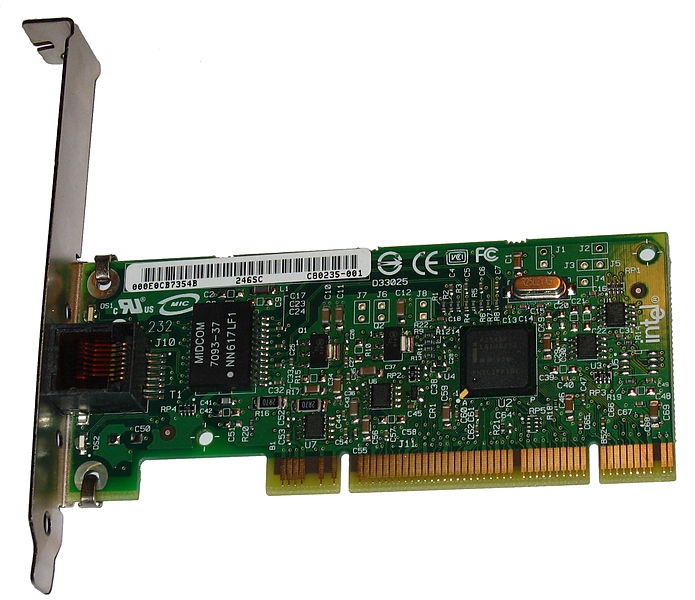
\includegraphics[width=0.5\textwidth]{base/Introduction/NIC.jpg}
 \caption{Сетевая карта}
 \label{base:introduction:components:nic:nicpic}
\end{figure}
\emph{Сетевая плата} (англ. \emph{network interface controller}) --- периферийное устройство, позволяющее компьютеру взаимодействовать с другими устройствами сети.
В настоящее время, особенно в персональных компьютерах, сетевые платы довольно часто интегрированы в материнские платы для удобства и удешевления всего компьютера в целом.

Доступ к сети может осуществляться как с помощью проводов, так и без них.
Для проводных сетевых карт характерно наличие разъёма 8P8C, внешне похожего на телефонный RJ-45.
Беспроводные платы вместо этого имеют антену, зачастую съёмную. Также на картах часто имеется светодиод, отображающий сетевую активность.
Серверные сетевые карты также имеют собственный процессор, снимающий нагрузку по обработке сетевого потока с центрального процессора.

Из значимых характеристик современных сетевых карт для домашнего пользования можно назвать следующие:
\begin{itemize}
 \item скорость передачи данных;
 \item интерфейс (шина подключения);
 \item поддержка различных стандартов, таких как 802.1p, 802.3x, и~т.\,д..
\end{itemize}

Сетевые карты обеспечивают передачу данных по сети, через них же осуществляется подключение к интернету. Подробнее сети, их организация и управление будут рассмотрены в \hyperref[base:networking]{главе \ref*{base:networking}}.

\subsubsection{Блок питания}\label{base:introduction:components:psu}
\begin{figure}[hb]
 \centering
 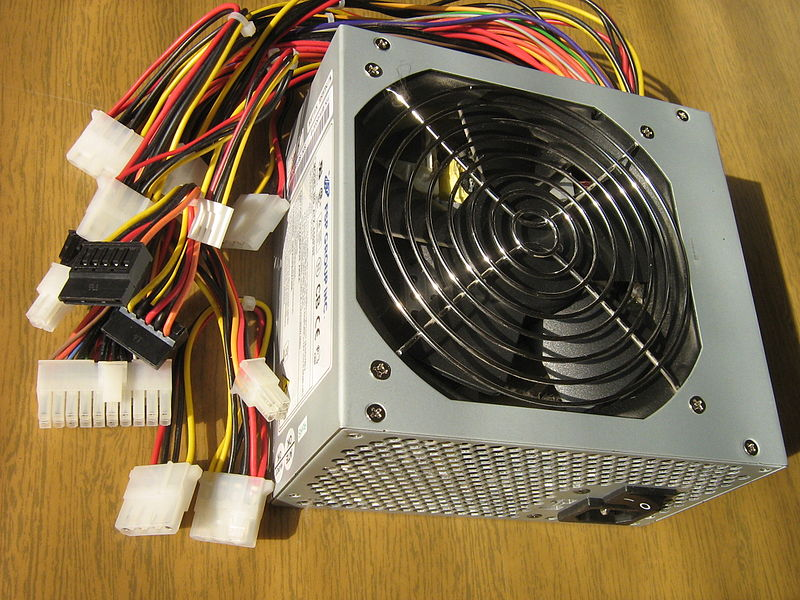
\includegraphics[width=0.5\textwidth]{base/Introduction/Power_supply_unit.jpg}
 \caption{Блок питания}
 \label{base:introduction:components:psupic}
\end{figure}
\emph{Блок питания} предназначен для снабжения узлов компьютера электрической энергией постоянного тока, путём преобразования сетевого напряжения до требуемых значений.

В некоторой степени блок питания также:
\begin{itemize}
 \item выполняет функции стабилизации и защиты от незначительных помех питающего напряжения;
 \item будучи снабжён вентилятором, участвует в охлаждении компонентов персонального компьютера.
\end{itemize}

Блок питания для настольного компьютера стандарта PC должен обеспечивать выходные напряжения $\pm 5$, $\pm 12$, $+3,3$ Вольт, а также $+5$ Вольт дежурного режима (англ. standby).
\begin{itemize}
 \item Основными силовыми цепями являются напряжения $+3,3$, $+5$ и $+12$ В. Причем, чем выше напряжение, тем большая мощность передается по данным цепям. Отрицательные напряжения питания ($−5$ и $−12$ В) допускают небольшие токи и в современных материнских платах в настоящее время практически не используются. 
 \begin{itemize}
  \item Напряжение $−5$ В использовалось только интерфейсом ISA и из-за фактического отсутствия этого интерфейса на современных материнских платах провод $−5$ В в новых блоках питания отсутствует.
  \item Напряжение $−12$ В необходимо лишь для полной реализации стандарта последовательного интерфейса RS-232, поэтому также часто отсутствует.
 \end{itemize}
 \item Напряжения $\pm 5$, $\pm 12$, $+3,3$, $+5$ В дежурного режима используются материнской платой. Для жёстких дисков, оптических приводов, вентиляторов используются только напряжения $+5$ и $+12$~В.
 \item Современные электронные компоненты используют напряжение питания не выше $+5$ Вольт. Наиболее мощные потребители энергии, такие как видеокарта, центральный процессор, северный мост подключаются через размещённые на материнской плате или на видеокарте вторичные преобразователи с питанием от цепей как $+5$ В, так и $+12$ В.
 \item Напряжение $+12$ В используется для питания наиболее мощных потребителей. Разделение питающих напряжений на $12$ и $5$ В целесообразно как для снижения токов по печатным проводникам плат, так и для снижения потерь энергии на выходных выпрямительных диодах блока питания.
 \item Напряжение $+3,3$ В в блоке питания формируется из напряжения $+5$ В, а потому существует ограничение суммарной потребляемой мощности по $\pm 5$ и $+3,3$ В.
\end{itemize}

Мощность, отдаваемая в нагрузку существующими БП, в значительной степени зависит от мощности компьютерной системы и варьируется в пределах от 50 (встраиваемые платформы малых форм-факторов) до 1800 Вт (большинство высокопроизводительных рабочих станций, серверов начального уровня или геймерских машин).
При этом стоит отметить, что на блоках питания указывается \emph{максимальная} мощность --- реально потребляемая почти всегда ниже этой величины.

Блок питания для ноутбуков и прочих мобильных компьютеров, как правило, применяется для зарядки аккумуляторных батарей, а также для обеспечения ноутбука питанием в обход аккумулятора.
По типу исполнения, блок питания ноутбука чаще всего является внешним элементом.
В виду практики выпускать БП под конкретную модель (серию) ноутбуков и учитывая тот факт, что характеристики разных моделей значительно разнятся, на внешние блоки питания нет единого стандарта, и сами БП обычно не взаимозаменяемы.
Также, производители ноутбуков часто используют различные разъёмы питания.

\subsubsection{Жёсткий диск}\label{base:introduction:components:hdd}
\begin{figure}
 \centering
 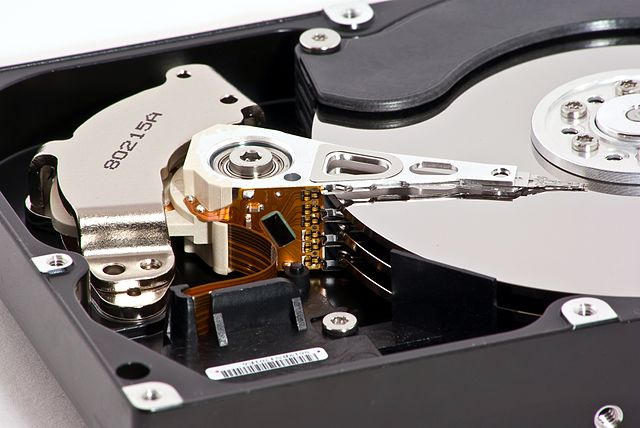
\includegraphics[width=0.5\textwidth]{base/Introduction/HDD.jpg}
 \caption{Разобранный жёсткий диск}
 \label{base:introduction:components:hddpic}
\end{figure}
\emph{Накопитель на жёстких магнитных дисках} (англ. \emph{hard disk drive}, также называемый <<\emph{винчестером}>>) является основным устройством долговременного хранения информации.
На нём хранится операционная система, загрузчик, пользовательские приложения и файлы.

Жёсткий диск состоит из \emph{гермозоны} и \emph{блока электроники}.
\begin{itemize}
 \item Гермозона включает в себя корпус из прочного сплава, собственно диски (пластины) с магнитным покрытием, а также блок головок с устройством позиционирования и электропривод шпинделя.
  \begin{itemize}
   \item Вопреки расхожему мнению, в подавляющем большинстве устройств внутри гермозоны нет вакуума.
    Одни производители делают её герметичной (отсюда и название) и заполняют очищенным и осушенным воздухом или нейтральными газами, в частности, азотом, а для выравнивания давления устанавливают тонкую металлическую или пластиковую мембрану.
    В этом случае внутри корпуса жёсткого диска предусматривается маленький карман для пакетика силикагеля, который абсорбирует водяные пары, оставшиеся внутри корпуса после его герметизации.
    Другие производители выравнивают давление через небольшое отверстие с фильтром, способным задерживать очень мелкие (несколько микрометров) частицы.
    Однако в этом случае выравнивается и влажность, а также могут проникнуть вредные газы.
    Выравнивание давления необходимо, чтобы предотвратить деформацию корпуса гермозоны при перепадах атмосферного давления и температуры, а также при прогреве устройства во время работы.
   \item Пылинки, оказавшиеся при сборке в гермозоне и попавшие на поверхность диска, при вращении сносятся на ещё один фильтр --- пылеуловитель.
   \item Блок головок --- пакет кронштейнов из упругой стали, обычно по паре на каждый диск.
    Одним концом они закреплены на оси рядом с краем диска. На других концах (над дисками) закреплены считывающие головки.
   \item Диски (пластины), как правило, изготовлены из металлического сплава.
    Большинство бюджетных устройств содержит одну или две пластины, но существуют модели с б\'{о}льшим числом пластин.
   \item Диски жёстко закреплены на шпинделе.
   Во время работы шпиндель вращается со скоростью несколько тысяч оборотов в минуту (3600, 4200, 5000, 5400, 5900, 7200, 9600, 10 000, 12 000, 15 000).
   При такой скорости вблизи поверхности пластины создаётся мощный воздушный поток, который приподнимает головки и заставляет их парить над поверхностью пластины.
   Форма головок рассчитывается так, чтобы при работе обеспечить оптимальное расстояние от пластины.
   Пока диски не разогнались до скорости, необходимой для <<взлёта>> головок, парковочное устройство удерживает головки в зоне парковки.
   Это предотвращает повреждение головок и рабочей поверхности пластин.
   \item Сепаратор (разделитель) --- пластина, изготовленная из пластика или алюминия, находящаяся между пластинами магнитных дисков и над верхней пластиной магнитного диска.
    Используется для выравнивания потоков воздуха внутри гермозоны.
   \item Устройство позиционирования (сервопривод) головок представляет из себя малоинерционный соленоидный двигатель.
    Оно состоит из неподвижной пары сильных постоянных магнитов, а также катушки на подвижном кронштейне блока головок.
  \end{itemize}
 \item Блок электроники:
  \begin{itemize}
   \item Интерфейсный блок обеспечивает сопряжение электроники жёсткого диска с остальной системой.
   \item Блок управления представляет собой систему управления, принимающую электрические сигналы позиционирования головок, и вырабатывающую управляющие воздействия приводом типа <<звуковая катушка>>, коммутации информационных потоков с различных головок, управления работой всех остальных узлов, приёма и обработки сигналов с датчиков устройства.
   \item Блок ПЗУ хранит программы для блоков управления и цифровой обработки сигнала, а также служебную информацию винчестера.
    Буферная память сглаживает разницу скоростей интерфейсной части и накопителя.
    Увеличение размера буферной памяти в некоторых случаях позволяет увеличить скорость работы накопителя.
   \item Блок цифровой обработки сигнала очищает считанный аналоговый сигнал и производит его декодирование.
  \end{itemize}
\end{itemize}

К основным характеристикам жёстких дисков можно отнести:
\begin{itemize}
 \item \emph{Интерфейс} (англ. \emph{interface}) --- техническое средство взаимодействия 2-х разнородных устройств, что в случае с жёсткими дисками является совокупностью линий связи, сигналов, посылаемых по этим линиям, технических средств, поддерживающих эти линии, и правил обмена.
  Современные серийно выпускаемые внутренние жёсткие диски чаще всего используют интерфейс SATA.
 \item \emph{Ёмкость} (англ. \emph{capacity}) --- количество данных, которые могут храниться накопителем.
  В отличие от принятой в информатике системы приставок, обозначающих кратную 1024 величину, производителями при обозначении ёмкости жёстких дисков используются величины, кратные 1000.
  Так, ёмкость жёсткого диска, маркированного как <<200 ГБ>>, составляет 186,2 ГиБ.
 \item \emph{Форм-фактор} (англ. \emph{dimension}).
  Почти все современные накопители для персональных компьютеров и серверов имеют ширину либо 3,5, либо 2,5 дюйма --- под размер стандартных креплений соответственно в настольных компьютерах и ноутбуках.
 \item \emph{Время произвольного доступа} (англ. \emph{random access time}) --- среднее время, за которое винчестер выполняет операцию позиционирования головки чтения/записи на произвольный участок магнитного диска.
  Диапазон этого параметра --- от 2,5 до 16 мс.
  Как правило, минимальным временем обладают серверные диски, самым большим из актуальных --- диски для портативных устройств.
 \item \emph{Скорость вращения шпинделя} (англ. \emph{spindle speed}) --- количество оборотов шпинделя в минуту.
  От этого параметра в значительной степени зависят время доступа и средняя скорость передачи данных.
  В настоящее время выпускаются винчестеры со следующими стандартными скоростями вращения: 4200, 5400 и 7200 (ноутбуки), 5400, 5900, 7200 и 10 000 (персональные компьютеры), 10 000 и 15 000 об/мин (серверы и высокопроизводительные рабочие станции).
  Увеличению скорости вращения шпинделя в винчестерах для ноутбуков препятствует гироскопический эффект, влияние которого пренебрежимо мало в неподвижных компьютерах.
 \item \emph{Надёжность} (англ. \emph{reliability}) --- определяется как среднее время наработки на отказ (MTBF).
 \item \emph{Скорость передачи данных} (англ. \emph{Transfer Rate}) при последовательном доступе:
  \begin{itemize}
   \item внутренняя зона диска: от 44,2 до 74,5 МиБ/с;
   \item внешняя зона диска: от 60,0 до 111,4 МиБ/с.  
  \end{itemize}
 \item \emph{Объём буфера} --- буфер это промежуточная память, предназначенная для сглаживания различий скорости чтения/записи и передачи по интерфейсу.
  В современных дисках он обычно варьируется от 8 до 64 МиБ.
\end{itemize}

Стоит также упомянуть предлагаемую замену жёстким дискам в виде \emph{твердотельных накопителей} (\emph{SSD}).
Они обладают огромным преимуществом по сравнению в жёсткими дисками:
\begin{itemize}
 \item Отсутствие движущихся частей;
 \item Высокая скорость чтения/записи, нередко превосходящая не только аналогичные параметры, но и пропускную способность интерфейса жёсткого диска;
 \item Низкое энергопотребление;
 \item Полное отсутствие шума из-за отсутствия движущихся частей и охлаждающих вентиляторов;
 \item Высокая механическая стойкость;
 \item Широкий диапазон рабочих температур;
 \item Стабильность времени считывания файлов вне зависимости от их расположения или фрагментации;
 \item Малые габариты и вес;
 \item Большой модернизационный потенциал как у самих накопителей, так и у технологий их производства.
 \item Намного меньшая чувствительность к внешним электромагнитным полям.
\end{itemize}
Однако, как и любая технология, они не лишены недостатков:
\begin{itemize}
 \item Главный недостаток SSD --- ограниченное количество циклов перезаписи.
  Обычная флеш-память позволяет записывать данные примерно 10 000 раз.
  Более дорогостоящие виды памяти --- более 100 000 раз.
  Для борьбы с неравномерным износом применяются схемы балансирования нагрузки.
  Контроллер хранит информацию о том, сколько раз какие блоки перезаписывались и при необходимости <<меняет их местами>>.
 \item Проблема совместимости SSD накопителей с устаревшими и даже многими актуальными версиями ОС семейства \foreignlanguage{english}{Windows}, которые не учитывают специфику SSD накопителей и дополнительно изнашивают их.
  Использование операционными системами механизма свопинга (подкачки) на SSD также, с большой вероятностью, уменьшает срок эксплуатации накопителя;
 \item Цена гигабайта SSD-накопителей существенно выше цены гигабайта HDD.
  К тому же, стоимость SSD прямо пропорциональна их ёмкости, в то время как стоимость традиционных жёстких дисков зависит от количества пластин и медленнее растёт при увеличении объёма накопителя.
 \item Применение в SSD-накопителях команды TRIM делает невозможным восстановление удалённой информации recovery-утилитами.
\end{itemize}

\subsubsection{Оптический привод}\label{base:introduction:components:opticaldrive}
Наконец, последним из частовстречающихся устройств внутри системного блока является \emph{оптический привод}.
Он использует лазер для чтения или записи данных с или на оптический диск.
Некоторые приводы могут только читать информацию с дисков, другие способны также записывать её.

Современные приводы читают и, если такая возможность поддерживается, записывают следующие типы оптических дисков:
\begin{itemize}
 \item CD-ROM (compact disk read-only memory);
 \item CD-R (recordable);
 \item CD-RW (rewritable);
 \item DVD-ROM (digital video disk);
 \item DVD-R;
 \item DVD+R;
 \item DVD-RW;
 \item DVD+RW;
\end{itemize}
Также встречаются устройства, способные читать или читать и записывать диски blu-ray.
% Вроде мало, но не думаю, что имеет смысл указывать что-то ещё. Хотя, если есть идеи...

\subsection{Монитор}\label{base:introduction:components:monitor}
Теперь, после того, как мы рассмотрели собственно компьютер, перейдём к подключаемым к нему устройствам.
Начнём с главного --- \emph{монитора}.
По своим функциям монитор схож с телевизором, за исключением источника сигнала --- в телевизорах сигнал поступает с антенны, а на компьютерные мониторы от видеокарты.
В некоторых случаях вместо монитора используется телевизор, или же подключается дополнительно для просмотра на нём фильмов.
Вообще в роли монитора может выступать любое устройство, способное воспроизводить видеосигнал; на конференциях, к примеру, часто подключают проекторы.

Самыми распространёнными типами экрана мониторов являются \emph{ЭЛТ} (англ.~\emph{CRT}) и \emph{ЖК} (англ.~\emph{LCD}).
\begin{itemize}
 \item Мониторы на электронно-лучевых трубках первыми использовались для вывода информации.
  До них единственным способом получить информацию из компьютера была печать, что приводило к большим задержкам и дополнительным расходам.
  ЭЛТ-технология широко применялась до начала 2000-х годов, однако затем её начали вытеснять более перспективные и экономичные технологии.
 \item Жидкокристаллические мониторы в настоящее время являются основным, бурно развивающимся направлением в технологии мониторов.
  К их преимуществам можно отнести: малые размер и масса в сравнении с ЭЛТ.
  У ЖК-мониторов, в отличие от ЭЛТ, нет видимого мерцания, дефектов фокусировки лучей, помех от магнитных полей, проблем с геометрией изображения и чёткостью.
  Энергопотребление ЖК-мониторов в зависимости от модели, настроек и выводимого изображения может как совпадать с потреблением ЭЛТ и плазменных экранов сравнимых размеров, так и быть существенно --- до пяти раз --- ниже.
  Энергопотребление ЖК-мониторов на 95\% определяется мощностью ламп подсветки или светодиодной матрицы подсветки ЖК-матрицы.
  Во многих мониторах 2007 года для настройки пользователем яркости свечения экрана используется широтно-импульсная модуляция ламп подсветки частотой от 150 до 400 и более герц.
  
  С другой стороны, ЖК-мониторы имеют и некоторые недостатки, часто принципиально трудноустранимые, например:
  \begin{itemize}
   \item В отличие от ЭЛТ, могут отображать чёткое изображение лишь в одном (<<штатном>>) разрешении.
    Остальные достигаются интерполяцией с потерей чёткости.
    Причем слишком низкие разрешения вообще не могут быть отображены на многих мониторах (например, 320×200).
    Многие из ЖК-мо\-ни\-то\-ров имеют сравнительно малый контраст и глубину чёрного цвета.
    Повышение фактического контраста часто связано с простым усилением яркости подсветки, вплоть до некомфортных значений.
    Широко применяемое глянцевое покрытие матрицы влияет лишь на субъективную контрастность в условиях внешнего освещения.
   \item Из-за жёстких требований к постоянной толщине матриц существует проблема неравномерности однородного цвета --- на некоторых мониторах есть неустранимая неравномерность передачи яркости, связанная с использованием блоков линейных ртутных ламп.
   \item Фактическая скорость смены изображения также остаётся ниже, чем у ЭЛТ и плазменных дисплеев.
    Современные технологии решают проблему скорости лишь частично.
   \item Зависимость контраста от угла обзора до сих пор остаётся существенным минусом технологии.
   \item Массово производимые ЖК-мониторы плохо защищены от повреждений.
    Особенно чувствительна матрица, незащищённая стеклом.
    При сильном нажатии возможна необратимая деградация.
   \item Существует проблема дефектных пикселей.
   Предельно допустимое количество дефектных пикселей, в зависимости от размеров экрана, определяется в международном стандарте ISO 13406-2 (в России --- ГОСТ Р 52324-2005).
   Стандарт определяет 4 класса качества ЖК-мониторов.
   Самый высокий класс --- 1, вообще не допускает наличия дефектных пикселей.
   Самый низкий --- 4, допускает наличие до 262 дефектных пикселей на 1 миллион работающих.
   \item Пиксели ЖК-мониторов деградируют, хотя скорость деградации наименьшая из всех технологий отображения, за исключением лазерных дисплеев, вообще не подверженных ей.
  \end{itemize}
\end{itemize}

Важнейшие характеристики ЖК-дисплеев:
\begin{itemize}
\item Тип матрицы --- технология, по которой изготовлен ЖК-дисплей;
 \item Класс матрицы --- по ISO 13406-2 подразделяются на четыре класса;
 \item Разрешение --- горизонтальный и вертикальный размеры, выраженные в пикселях.
  В отличие от ЭЛТ-мониторов, ЖК имеют одно фиксированное разрешение, остальные достигаются интерполяцией;
 \item Размер точки (размер пикселя) --- расстояние между центрами соседних пикселей.
  Непосредственно связан с физическим разрешением;
 \item Соотношение сторон экрана (пропорциональный формат) --- отношение ширины к высоте (5:4, 4:3, 3:2 (15:10), 8:5 (16:10), 5:3 (15:9), 16:9 и др.);
 \item Видимая диагональ --- размер самой панели, измеренный по диагонали.
  Площадь дисплеев зависит также от формата: монитор с форматом 4:3 имеет большую площадь, чем с форматом 16:9 при одинаковой диагонали;
 \item Контрастность --- отношение яркостей самой светлой и самой тёмной точек при заданной яркости подсветки.
  В некоторых мониторах используется адаптивный уровень подсветки с использованием дополнительных ламп, приведённая для них цифра контрастности (так называемая динамическая) не относится к статическому изображению.
 \item Яркость --- количество света, излучаемое дисплеем, обычно измеряется в канделах на квадратный метр.
 \item Время отклика --- минимальное время, необходимое пикселю для изменения своей яркости.
  Составляется из двух величин: 
  \begin{itemize} 
   \item Время буферизации (input lag).
    Высокое значение мешает в динамичных играх; обычно умалчивается; измеряется сравнением с кинескопом в скоростной съёмке.
    Сейчас в пределах 20--50 мс; в отдельных ранних моделях достигало 200 мс;
   \item Время переключения --- именно оно указывается в характеристиках монитора.
    Высокое значение ухудшает качество видео; методы измерения неоднозначны.
    Сейчас практически во всех мониторах заявленное время переключения составляет 2--6 мс.
  \end{itemize}
 \item Угол обзора --- угол, при котором падение контраста достигает заданного, для разных типов матриц и разными производителями вычисляется по-разному, и часто не подлежит сравнению.
  Некоторые производители указывают в тех. параметрах своих мониторов углы обзора такие, к примеру, как: CR 5:1 --- $176/176^{\circ}$, CR 10:1 --- $170/160^{\circ}$.
  Аббревиатура CR (contrast ratio) обозначает уровень контрастности при указанных углах обзора относительно перпендикуляра к экрану.
  При углах обзора $170^{\circ}/160^{\circ}$ контрастность в центре экрана снижается до значения не ниже чем 10:1, при углах обзора $176^{\circ}/176^{\circ}$ не ниже чем до значения 5:1.
\end{itemize}

\subsection{Периферия}\label{base:introduction:components:peripheral}
\subsubsection{Клавиатура}\label{base:introduction:components:peripheral:keyboard}
% Это уже откровенная паста с википедии, но лучшего изложения придумать сложно
\begin{figure}
 \centering
 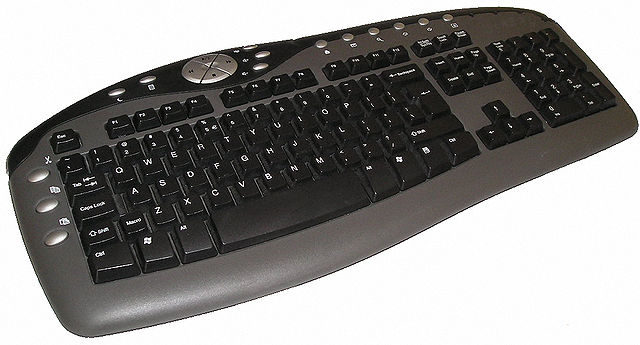
\includegraphics[width=0.5\textwidth]{base/Introduction/Keyboard.jpg}
 \caption{Клавиатура}\label{base:introduction:components:peripheral:keyboardpic}
\end{figure}
Компьютерная клавиатура --- одно из основных устройств ввода информации от пользователя в компьютер.
Обычно компьютерная клавиатура имеет 101--105 клавиш.

По своему назначению клавиши на клавиатуре делятся на шесть групп:
\begin{enumerate}
 \item функциональные;
 \item алфавитно-цифровые;
 \item управления курсором;
 \item цифровая панель;
 \item специализированные;
 \item модификаторы.
\end{enumerate}

Двенадцать функциональных клавиш расположены в самом верхнем ряду клавиатуры.
Ниже располагается блок алфавитно-цифровых клавиш.
Правее этого блока находятся клавиши управления курсором, а с самого правого края клавиатуры --- цифровая панель.

\paragraph{Алфавитно-цифровой блок}
К алфавитно-цифровому блоку относятся клавиши для ввода букв, цифр, знаков пунктуации и арифметических действий, специальных символов.
В стандартной клавиатуре этот блок включает 47 клавиш.

Клавиши алфавитно-цифрового блока делятся по рядам и по зонам.
Нижний ряд блока находится над клавишей <<пробел>> (\Spacebar) и клавишами-модификаторами \Ctrl, \Alt, \AltGr.
Он считается первым.
Выше --- второй, в методе слепой десятипальцевой печати также называемый <<домашним>> рядом.
Ещё выше --- третий.
Самый верхний ряд клавиш блока --- четвёртый --- в латинской раскладке QWERTY не содержит клавиш для ввода букв, но включает все клавиши ввода цифр.
По этой причине его часто называют цифровым рядом.

Зоной называется совокупность клавиш, закреплённых в методе слепой десятипальцевой печати за пальцами каждой из рук.
Нумерация зон идёт слева направо.

Результат действия алфавитно-цифровых клавиш зависит от регистра (нижний---верхний) и уровня (первый---второй) в котором осуществляется нажатие этих клавиш.

\paragraph{Клавиши-модификаторы}
К клавишам-модификаторам относятся клавиши \Shift, \Ctrl, \keystroke{CapsLock}, \Alt и \AltGr (правый Alt).
Они предназначены для изменения (модификации) действий других клавиш.
Включение верхнего регистра клавиш (при отключённом \keystroke{CapsLock}) осуществляется нажатием и удержанием клавиши \Shift. Нажатие и удержание клавиши \AltGr используется для перехода на второй уровень клавиатуры.
Клавиши-модификаторы используются наиболее часто, поэтому они имеют увеличенный размер.
К тому же клавиши \Shift и \Ctrl продублированы по обеим сторонам блока алфавитно-цифровых клавиш.

\paragraph{Функциональные клавиши}
На верхней части клавиатуры, а иногда в другом месте, располагается блок так называемых функциональных клавиш --- от \keystroke{F1} до \keystroke{F12}.
Функции этих клавиш определяются программой и операционной системой, с которой пользователь работает в данный момент.
Часто программы устанавливают те или иные функции и для комбинаций функциональных клавиш с клавишами \Shift, \Ctrl и \Alt.
Во многих программах при нажатии \keystroke{F1} на экран выводится встроенный справочник по программе (часто уже открытый на странице, соответствующей режиму программы, в котором она находится).

\paragraph{Цифровая панель}
Основное назначение клавиш цифровой панели --- дублирование функций клавиш алфавитно-цифрового блока в части ввода цифр и арифметических операторов.
Клавиши этой панели более удобны для ввода цифр и арифметических операторов, нежели клавиши алфавитно-цифрового блока.

\paragraph{Мультимедийные клавиши}
Многие современные клавиатуры помимо стандартного набора снабжаются дополнительными клавишами (как правило, другого размера и формы), которые предназначены для упрощённого управления некоторыми основными функциями компьютера:
\begin{itemize}
 \item управление громкостью звука: громче, тише, включить или выключить звук;
 \item управление лотком в приводе для компакт-дисков: извлечь диск, принять диск;
 \item управление аудиопроигрывателем: играть, остановить, поставить на паузу, промотать аудиозапись вперёд или назад, перейти к следующей или предыдущей аудиозаписи;
 \item управление сетевыми возможностями компьютера: открыть почтовую программу, открыть браузер, показать домашнюю страницу, двигаться вперёд или назад по истории посещённых страниц, открыть поисковую систему;
 \item управление наиболее популярными программами: открыть калькулятор, открыть файловый менеджер;
 \item управление состоянием окон операционной системы: свернуть окно, закрыть окно, перейти к следующему или к предыдущему окну;
 \item управление состоянием компьютера: перевести в ждущий режим, перевести в спящий режим, пробудить компьютер, выключить компьютер.
\end{itemize}

Так как многие из этих функций относятся к сфере мультимедиа, то такие клавиатуры часто называются <<мультимедийными клавиатурами>>.

Фирменные драйверы таких клавиатур, как правило, не предоставляют пользователям возможности управлять назначением большинства дополнительных клавиш, а также не дают возможности определять дополнительные сочетания из нескольких клавиш и назначать им новые специальные функции.
Однако, эта проблема может быть решена при помощи независимых универсальных драйверов от сторонних разработчиков.

\subsubsection{Мышь}\label{base:introduction:components:peripheral:mouse}
\begin{figure}
 \centering
 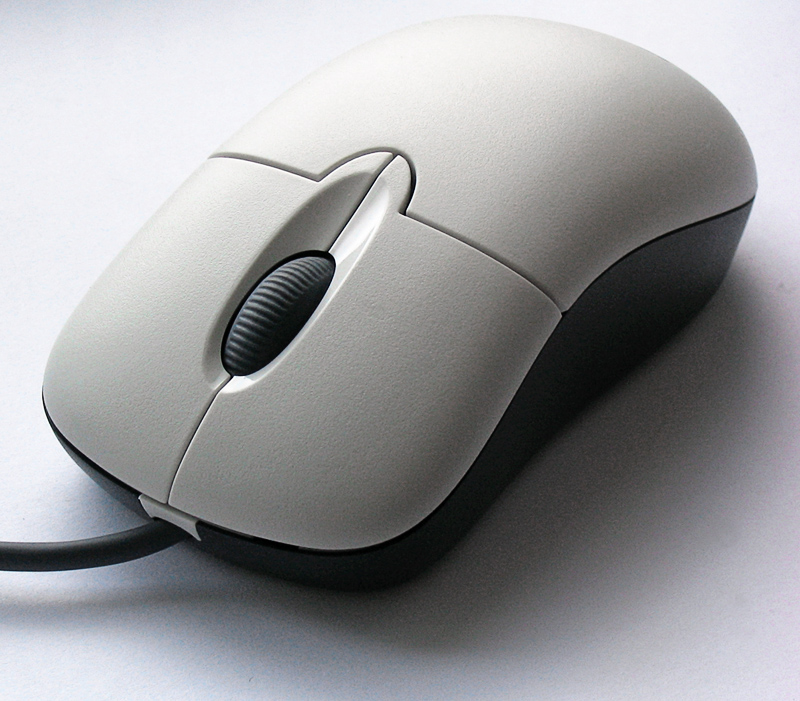
\includegraphics[width=0.5\textwidth]{base/Introduction/Mouse.jpg} 
 \caption{Компьютерная мышь}\label{base:introduction:components:peripheral:mousepic}
\end{figure}
\emph{Манипулятор типа <<мышь>>} --- второе по частоте использования устройство ввода, одно из основных устройств управления компьютером.

Принцип действия заключается в передаче компьютеру данных о перемещении или нажатии/отпускании кнопок.
Данный тип манипуляторов обладает широкими возможностями управления и позиционирования.
Программа, работающая на компьютере, в ответ на перемещение мыши производит на экране действие, отвечающее направлению и расстоянию этого перемещения.
В универсальных интерфейсах (например, в оконных) с помощью мыши пользователь управляет специальным курсором --- указателем --- манипулятором элементами интерфейса.

Кнопки --- основные элементы управления мыши, служащие для выполнения основных манипуляций: выбора объекта (нажатиями), активного перемещения (то есть перемещения с нажатой кнопкой, для рисования или обозначения начала и конца отрезка на экране, который может трактоваться как диагональ прямоугольника, диаметр окружности, исходная и конечная точка при перемещении объекта, выделении текста и~т.\,п.).
Кнопки называют по положению --- левая (под указательный палец правши), правая и средняя, для трёхкнопочной мыши.

Дополнительные кнопки на некоторых мышах служат различным целям --- настройка чувствительности, навигация и~т.\,д..

\subsubsection{Джойстик}\label{base:introduction:components:peripheral:joystick}

\subsubsection{Колонки}\label{base:introduction:components:peripheral:loudspeaker}

\subsubsection{Веб-камера}\label{base:introduction:components:peripheral:webcam}

\subsubsection{Микрофон}\label{base:introduction:components:peripheral:microphone}

\subsection{Принтеры, сканеры и МФУ}\label{base:introduction:components:printers}
\subsubsection{Принтер}\label{base:introduction:components:printers:printer}

\subsubsection{Сканер}\label{base:introduction:components:printers:scanner}

\subsubsection{Копировальный аппарат}\label{base:introduction:components:printers:copier}

